% !TeX root = manifold.tex
% author: buwailee@nmhs
\chapter{流形与纤维丛}
\section{基础}

\begin{para}
一个局部$n$维欧几里得空间是一个Hausdorff空间$M$满足,对每一个点$p\in M$,存在一个$p$的邻域$U\subset M$和一个同胚$\varphi:U\to V$,其中$V$是一个$\rr^n$中的开集。这个同胚有时候被称为一个坐标、坐标映射等,而资料$(U,\varphi)$被称为一个\idx{坐标卡}。坐标$\varphi$经常写成分量形式,$\varphi=(x^1$, $\dots$, $x^n)$,其中$x^i:U\to \rr$. 

方便起见,我们经常在一点$p\in M$附近选择坐标卡$(U,\varphi)$使得$\varphi(p)=0$,否则只需复合一个欧氏空间的平移,它显然是光滑的。这样的坐标卡被称为以$p$为中心的坐标卡。
\end{para}

虽然欧氏空间是Hausdorff的,但是它可以粘起来得到一个非Hausdorff的拓扑空间。如下图所示:
\begin{center}
\includegraphics[width=0.7\textwidth,bb=0 0 561 68]{1.png}
\end{center}
将除了原点的两个实直线粘起来得到的拓扑空间,对于两个原点,它们是不能通过开集分离的。这个例子特别典型,被称为具有双重原点的直线。这样的东西我们多半不喜欢,在代数几何上,我们也会引入一个类似于Hausdorff性的分离性\footnote{代数几何上处理的对象(概形)的拓扑一般很差,特别地,几乎不会是Hausdorff的,所以那里的分离性不是Hausdorff性。}来避免这样的东西出现。

定义中,局部同胚可以选为同胚于欧式空间中的一个开球。实际上,若我们在$p\in M$处有了一个局部同胚$\varphi:U\to V$,而$V$是欧式空间中的开集,所以必然有包含$\varphi(p)$的一个开球$W$包含其中,将$\varphi^{-1}$限制在$W$上,然后取逆就到了$p$的一个同胚于欧式空间开球的邻域。注意到开球实际上也是(光滑)同胚于整个欧式空间$\rr^n$的,所以说流形局部同胚于整个欧式空间也没什么问题。具体的取什么同胚,还是依所处语境来做判断为好。一般来说,将这个开集取成连通的是方便的。

此外,局部$n$维欧几里得空间是局部紧的,这是因为一方面他是Hausdorff的,另一方面它局部同胚于欧式空间。

\begin{para}
局部欧几里得空间$M$上的一个光滑微分结构$\mathscr{F}$是这样一族坐标卡$(U_\alpha,\varphi_\alpha)$,满足:$\{U_\alpha\}$构成$M$的开覆盖,$\varphi_\alpha\circ\varphi^{-1}_\beta|_{U_\alpha\cap U_\beta}$是光滑映射,后者被称为坐标卡的相容性条件。此外,如果有一个坐标卡$(U,\varphi)$和每一个坐标卡都相容,那么可以推断出他在$\mathscr{F}$中,这样的微分结构被称为极大微分结构。极大微分结构当然不一定是唯一的,不过我们不担心这个,因为我们往往是固定一个微分结构来研究流形的几何,下面假设出现的微分结构总是极大的。

设$(M,\mathscr{F})$和$(N,\mathscr{G})$是两个光滑流形,连续函数$f:M\to N$被称为一个\idx{光滑映射},如果$\psi\circ f\circ \varphi^{-1}$是一个光滑函数对任意的$\mathscr{F}$中的坐标卡$(U,\varphi)$和$\mathscr{G}$中的坐标卡$(V,\psi)$成立。由于欧式空间之间的光滑函数的复合依然是光滑的,所以光滑的定义是不依赖于坐标卡的选取的。

这样,光滑流形就构成了一个范畴,其中态射是流形间的光滑映射。他是拓扑空间范畴的子范畴。
\end{para}

从此以后,我们对一个固定的流形$(M,\mathscr{F})$,常常会略去他的微分结构,只写作$M$. 对于一个光滑流形$M$的非空开子集$U$,显然,他有继承自$M$的一个拓扑结构和微分结构,所以$U$也是一个光滑流形。很容易看到,$\rr^n$是一个光滑流形,所以我们已经得到了一类光滑流形,$\rr^n$的开子集。比如把$n\times n$矩阵放入$\rr^{n^2}$内,那么行列式不为零的那些矩阵就构成一个光滑流形,记作$\operatorname{GL}(n,\rr)$,称作一般线性群。

特别地,$\rr$也是一个光滑流形。我们称光滑映射$f:M\to \rr$是一个$M$上的光滑函数。光滑函数$f$限制在$U\subset M$上也是一个光滑函数$f|_U$.

\begin{para}[光滑函数芽]
设$M$是一个光滑流形,$U\subset M$上的光滑函数的集合记作$\calf(U)$,$\calf$被称为$M$上的光滑函数\idx{层}。由于可以逐点定义加法和乘法,所以$\calf(U)$拥有$\rr$-代数结构。设$p\in M$,我们定义如下等价关系:设$U$和$V$都是$p$的邻域,以及$f\in \calf(U)$和$g\in \calf(V)$,如果在一个$W\subset U\cap V$上,$f|_W=g|_W$,则$f\sim g$. 所有这样的等价类记作$\calf_p$,称为$p$处的光滑函数\idx{茎},他的代表元素可以写成$f_p=\langle U,f\rangle$,称为\idx{芽}. 显然$\calf_p$有继承自$\calf(U)$的自然的$\rr$-代数结构。上述过程也可以用colimit表示为
\[
\calf_p={\varinjlim}_{U\ni p}\calf(U),
\]
其中$p$的邻域以包含形成归纳系。
\end{para}

我们下面研究$\calf_p$的代数结构。

\begin{pro}
$\calf_p$是一个局部环,它唯一的极大理想由所有$\langle U,f\rangle \in \calf_p$且$f(p)= 0$的元素构成了,记作$\mm_p$. 此外,$\calf_p/\mm_p\cong \rr$.
\end{pro}

\begin{proof}
设$\langle U,f\rangle$不在这个理想内的。由于$f(p)\neq 0$,那么适当缩小$U$到$V$,由$f$的连续性,总可以找到$V$使得$f|_V$处处不为零,这样$\langle V,1/f|_V\rangle$便是$\langle U,f\rangle$的一个逆。因此这个理想就是$\calf_p$唯一的极大理想,$\calf_p$是一个局部环。最后我们来证明$\calf_p/\mm_p\cong \rr$. 对每一个芽$f_p\in\calf_p$,都成立$f_p=f_p-f(p)+f(p)$,在$\calf_p/\mm_p$中看,他和$f(p)\in\rr$也就没区别了。
\end{proof}

为了在细致研究流形上光滑函数局部的结构,我们需要下面的这个引理。

\begin{lem}\label{lem:1.1.5}
设$f:U\to \rr$光滑,则存在一个以$p$为中心的坐标卡$(V,\varphi)$使得对任意的$q\in V$成立
\[
	f(q)=f(p)+\frac{\partial f\circ \varphi^{-1}}{\partial x^i}(p)x^i(q)+g_{ij}(q)x^i(q)x^j(q),
\]
其中$g_{ij}$在$V$上光滑。
\end{lem}

以后我们将那个偏微分$\partial f\circ \varphi^{-1}/\partial x^i (p)$简记作$\partial_i f(p)$.

\begin{proof}
完全局部的结果,让我们先证明欧氏空间的对应物:设$f:\rr^n\to \rr$光滑,则
\[
	f(x)=f(0)+\partial_if(0)x^i+g_{ij}(x)x^ix^j,
\]
其中$g_{ij}$光滑。

实际上,利用微积分基本定理
\[
	f(x)-f(0)=\int_0^1f'(tx)\dd t=\int_0^1\partial_i f(tx)x^i\dd t=h_i(x)x^i,
\]
可以得到$h_i(0)=\partial_i f(0)$,于是
\[
	f(x)=f(0)+h_i(x)x^i.
\]
同理,对$h_i$也有
\[
	h_i(x)=\partial_i f(0)+g_{ij}(x)x^j.
\]
所以
\[
	f(x)=f(0)+\partial_i f(0)x^i+g_{ij}(x)x^ix^j.
\]
最后,利用坐标卡翻译到流形上即可。
\end{proof}

类似地,同样使用微积分基本定理,我们还能证明下面这个引理。

\begin{lem}\label{lem:1.5}
设$I=(-\epsilon,\epsilon)$是一个区间,而$f(t,p)$是$I\times M$上的一个光滑函数。如果$f(0,p)=0$对任意的$p\in M$都成立,则存在一个函数$g(t,p)$使得$f(t,p)=tg(t,p)$,且对每一个$p\in M$,我们有$g(0,p)=f'(0,p)$,其中$f'=\partial_t f$.
\end{lem}

\begin{proof}
	直接定义
	\[
	g(t,p)=\int_0^1 f'(ts,p)\dd s
	\]
	即可。注意到
	\[
	tg(t,p)=\int_0^tf'(st,p)\dd (st)=\int_0^tf'(s,p)\dd s=f(t,p)-f(0,p)=f(t,p),
	\]
	同时两边对$t$在$t=0$处求导,就得到了$g(0,p)=f'(0,p)$.
\end{proof}

\begin{para}[余切空间]
设$p\in M$,$p$处的茎为$\calf_p$,他的极大理想为$\mm_p$,此时$p$处的\idx{余切空间}被定义为自然的矢量空间$T_p^*M:=\mm_p/\mm_p^2$. 余切空间的元素被称为\idx{余切矢量}。
\end{para}

可以看到,$\mm_p/\mm_p^2$确实是一个矢量空间。首先它显然是一个$\calf_p$-模,然后任取$a\in \mm_p$,由于$a\mm_p/\mm_p^2=0$,所以$\mm_p/\mm_p^2$是一个$\calf_p/\mm_p$-模,即$\rr$-矢量空间。这样定义的余切空间,可以看到,是所有的那些一阶小量构成的集合,即其中的元素为“\idx{微分}”。

\begin{para}[微分算子]
典范商同态$\mm_p\to \mm_p/\mm_p^2$特别重要,我们记作$\dd_p$. 然而,只处理极大理想中的元素并不是很方便,所以,对$p$处的常值芽$a$(即$\langle U,a\rangle\in\calf_p$,其中$a$在$U$内为常值函数),我们补充定义$\dd_pa=0$,这样就得到了新的算子$\dd_p:\calf_p\to T_p^*M$,它被称为\idx{微分}算子。
\end{para}

方便起见,我们用$\dd_p(f)$, $\dd_pf$或者$\dd f(p)$来记$\dd_p(f_p)$,如果$p$不需要指出,甚至有时候会记作$\dd f$. 

\begin{pro}[Leibniz法则]
$\dd_p (fg)=f(p)\dd_pg+\dd_pf g(p)$.
\end{pro}

% 对于微分算子,Leibniz法则是熟知且常用的。

\begin{proof}
由于
\[
	(fg)_p-f(p)g(p)=\bigl(f_p-f(p)\bigr)\bigl(g_p-g(p)\bigr)+f(p)\bigl(g_p-g(p)\bigr)+\bigl(f_p-f(p)\bigr)g(p),
\]
其中第一项属于$\mm_p^2$,所以
\[
\dd_p (fg)=f(p)\dd_p\bigl(g-g(p)\bigr)+\dd_p\bigl(f-f(p)\bigr)g(p)=f(p)\dd_pg+\dd_pf g(p).\qedhere
\]
\end{proof}

\begin{para}[拉回映射]
设$f:M\to N$是一个光滑映射,上面的光滑函数层分别为$\calf$和$\calg$. 任取$\varphi\in \calg(V)$,可以通过$f^*\varphi=\varphi\circ f$定义$f^*\varphi\in \calf(f^{-1}(V))$. 显然,$(f\circ g)^*=g^*\circ f^*$.

局部地,可以考虑两个流形余切空间之间的映射。设$\langle V,\varphi\rangle\in \calg_{f(p)}$,于是$\langle f^{-1}(V),\varphi\circ f\rangle\in \calf_p$,所以$f^*$诱导了一个$\rr$-代数同态$f^*_p:\calg_{f(p)}\to \calf_p$,特别地,可以看到$f^*_p:\mm_{f(p)}\to \mm_{p}$以及$f^*_p:\mm^2_{f(p)}\to \mm^2_{p}$. 因此$f^*$诱导了一个线性映射\footnote{这里我们滥用一下记号。}
\[
	f^*_p:T_{f(p)}^*N\to T_p^*M.
\]

由$(f\circ g)^*=g^*\circ f^*$,容易得到$(f\circ g)^*_p=g^*_p\circ f^*_{g(p)}$. 并且,$\id^*_p=\id_{T_p^*M}$,所以如果$f:M\to N$是同胚,则$f_p^*:T_{f(p)}^*N\to T_p^*M$是同构。
\end{para}

对于一个矢量空间来说,维数是肯定要关注的不变量。并且在一般意义上,维数应该是局部概念。我们有如下命题:

\begin{pro}
设$p\in M$,$M$是一个$n$维流形,则$\dim T_p^*M=n$. 如果选定以$p$为中心的一个局部坐标$\varphi=(x^1$, $\dots$, $x^n)$,则$T_p^*M$的基可以选作$\{\dd_p x^i\}$.
\end{pro}

\begin{proof}
由于选取不同的局部坐标都是通过同胚联系的,从拉回映射那里看到,同胚诱导了余切空间的同构,所以维数并不会发生改变。所以我们可以选定一组局部坐标来算维数。现在给定一个以$p$为中心的局部坐标$\varphi=(x^1$, $\dots$, $x^n)$,首先指出,$x^i$在点$p$处是一个一阶小量但不是一个二阶小量,即$x^i_p\not\in \mm^2$,或者说$\dd_p x^i\neq 0$.

从Lemma \ref{lem:1.1.5},$\mm_p$作为$\calf_p$-模,它可以由$\{x^i_p\}$和$\{x^i_px^j_p\}$生成。因此,$\mm_p^2$可以由$\{x^i_px^j_{p}\}$, $\{x^i_px^j_{p}x^k_p\}$, $\{x^i_px^j_{p}x^k_px^l_p\}$生成。如果$x^i_p\in \mm_p^2$,则
\[
	x^i_p=(a_{jk})_px^j_px^k_p+(b_{rst})_p x^r_px^s_px^t_p+(c_{jkrs})_p x^j_px^k_px^r_px^s_p.
\]
这就意味着,在$p$的某个小邻域$U$中成立等式
\[
	x^i=a_{jk}x^j x^k +b_{rst} x^r x^s x^t +c_{jkrs} x^j x^k x^r x^s .
\]
其中$a_{jk}$, $b_{rst}$, $c_{jkrs}$为$p$附近的光滑函数。利用坐标映射,可以在$\rr^n$的$0$附近的小邻域$\varphi(U)$中考虑这个等式。将两边对$x^i$求个导,然后令所有的$\{x^i\}$都趋向于$0$,即得到了矛盾。所以$\dd_p x^i\neq 0$.

同样,从Lemma \ref{lem:1.1.5},如果$f_p\in \calf_p$,则
\[
	f_p=f(p)+\partial_i f(p)x^i_p+(g_{ij})_p x^i_px^j_p.
\]
所以
\begin{equation}
\label{c1:e1}
	\dd_p f=\partial_i f(p)\dd_p x^i.
\end{equation}
这样所有的$T_p^*M=\mm_p/\mm_p^2$中的元素都可以由$\dd_px^i$展开,他们都是非零的,而且容易证明是线性无关的,所以这是$T_p^*M$的一组基,余切空间的维数计算完毕。
\end{proof}

\begin{para}[切空间]
设$p\in M$,$M$是$n$维光滑流形,则\idx{切空间}$T_pM$被定义为余切空间$T_p^*M$的对偶空间。切空间的元素被称为\idx{切矢量}。由于余切空间是有限维的,他的对偶空间也和他有着相同的维度,即$n$维。
\end{para}

对于有限维空间,对偶空间的对偶空间就是原本的空间。在这里,这就是说可以将余切空间的矢量看成切空间矢量的线性函数:设$\dd_p f\in T_p^*M$和$v\in T_pM$,定义$\dd_p f(v):=v(\dd_p f)$.

类似于我们将$\dd_p$扩张到了$\mathcal{F}_p$上,下面我们将一个切矢量扩张到$\calf_p^*$上面去。设$f$是在$p$附近的光滑函数,而$v\in T_pM$,可以通过$D_v(f_p):=v(f_p-f(p))$定义线性映射$i_p:v\mapsto D_v\in \calf_p^*$,他是一个单射。注意到$(fg)_p=f_pg_p$,所以
\[
	\begin{aligned}
		D_v(f_pg_p)&=v(f_pg_p-f(p)g(p))\\
		&=v\bigl((f_p-f(p))(g_p-g(p))+f(p)(g_p-g(p))+(f_p-f(p))g(p)\bigr)\\
		&=f(p)D_v(g_p)+D_v(f_p)g(p),
	\end{aligned}
\]
我们将满足这条性质(Leibniz法则)的线性映射$D_v\in \calf_p^*$称为$p$处的导子。

\begin{lem}
$p$处的所有导子构成的空间与$T_pM$典范同构。
\end{lem}

\begin{proof}
记$p$处的所有导子构成的空间为$V_p$. 任取导子$D\in V_p$,由于$D(1)=D(1\times 1)=2D(1)$,所以$D(1)=0$,继而靠着$D$的线性性,对于常值函数的芽$a$来说,$D(a)=aD(1)=0$。因为每一个$\calf_p$中的元素$f_p$都可以写成$f_p-f(p)+f(p)$的形式,所以$D(f_p)=D(f_p-f(p))$,这就是说,一个导子的性质完全由他在$\mm_p$上的值决定,这种关系是一对一的,即$\pi_p:D\mapsto D|_{\mm_p}$是一个线性同构。

同时,设$f_p$, $g_p\in \mm_p$,则$\pi_p(D)(f_pg_p)=f(p)\pi_p(D)(g_p)+g(p)\pi_p(D)(f_p)=0$,于是$\pi_p(D)(\mm_p^2)=0$,所以,$\pi_p(D)\in T_pM$,即$D|_{\mm_p}$是一个切矢量,因此导子$D$完全由一个切矢量$D|_{\mm_p}=\pi_p(D)$决定。这样,$i_p:T_pM\to V_p$也是一个满射,所以他是一个同构。当然我们也可以直接计算验证$\pi_p\circ i_p=\id_{T_pM}$以及$i_p\circ \pi_p=\id_{V_p}$.
\end{proof}

因为有这个同构,所以以后我们用$T_pM$来标记导子构成的矢量空间,一个导子才是一个切矢量。这样的好处是,我们在具体计算的时候,可以直接在$\calf_p$上进行而非$\mm_p$上,特别地,现在对于一个切向量$v$来说,成立$\dd_pf(v)=v(f_p)$,这是因为对一个导子$v$来说$v(f_p)=v(\dd_pf)$.

\begin{para}[推前映射]
设$f:M\to N$是一个光滑映射,定义它在$p\in M$处的导数为$T_pf=f_{*p}:T_pM\to T_{f(p)}N$使得对任意的$v\in T_p M$和任意的$g_{f(p)}\in \mm_{f(p)}$成立$(f_{*p}v)(g_{f(p)})=v(f_p^*g_{f(p)})=v((g\circ f)_p)$.
\end{para}

通过坐标卡上的同胚$\varphi$,我们用$\partial_i$来标记$\varphi^{-1}_{*p}(e_i)$,这显然是$T_pM$处的一组基。特别地,如果$M=\rr^n$,为方便处理,可以通过等同$\partial_i$和标准基$e_i$来等同$T_p\rr^n$和$\rr^n$. 选定一个局部坐标$\varphi=(x^1$, $\dots$, $x^n)$,因为
\[
	\dd_p x^i(\partial_j)=\partial_jx^i(p)=\delta^i_j,
\]
所以$\dd_p x^i$就是$\partial_i$的对偶基。

\begin{pro}对于实值光滑函数和矢量值光滑函数,我们可以计算出推前映射$f_{*p}$:
\begin{compactenum}
\item 设$f$是在$p$附近的光滑函数,则$f_{*p}=\dd_p f$. 
\item 设$f:M\to \rr^n$是一个流形$M$上的矢量值光滑函数,选取$e_i$和$\dd x^j$为基,则$f_{*p}:T_pM\to \rr^n$的矩阵写作:
\[
	(f_{*p})^{i}_{\phantom{i}j}=\partial_j f^i(p),
\]
此即$f$的Jacobian.
\end{compactenum}
\end{pro}

\begin{proof}
第一点,任取$v\in T_pM$. 因为$f_{*p}:T_pM\to T_{f(p)}\rr=\rr$,所以$f_{*p}(v)$是一个数,故而
\[
	f_{*p}(v)=f_{*p}(v)(\id_{\rr})=v\bigl((\id_{\rr}\circ f)_p\bigr)=v(f_p)=\dd_p f(v).
\]
因为对所有的切矢量$v$都成立上式,所以$f_{*p}=\dd_p f$.

第二点,设$f:M\to \rr^n$是一个流形$M$上的矢量值光滑函数,则第$i$个分量$f^i:M\to \rr$是一个光滑函数,那么$f_{*p}=\dd_pf^i e_i$,其中$e_i$是$\rr^n$的标准基。再由
$\dd_pf^i=\partial_j f^i(p) \dd x^j$,
所以,当选取$e_i$和$\dd x^j$为基时,$f_{*p}$写成矩阵即$(f_{*p})^{i}_{\phantom{i}j}=\partial_j f^i(p)$.
\end{proof}

\begin{para}[复合函数求导法则]
$(f\circ g)_{*p}=f_{*g(p)}\circ g_{*p}$. 抽象表现出来是线性映射复合,表现在矩阵(即Jacobian)上就是两个矩阵相乘。
\end{para}

\begin{para}\label{f*d=df*}
利用复合公式,设$f:M\to N$是光滑映射而$g$是$N$上的光滑函数,则
\[
	(g\circ f)_{*p}=(f^*g)_{*p}=\dd_p(f^*g),\quad (g\circ f)_{*p}=f_{*p}g_{*f(p)}=f_{*p}\left(\dd_{f(p)}g \right),
\]
所以$f^*_p\bigl(\dd_{f(p)}g\bigr)=\dd_{p}(f^*g)$. 所以,拉回和微分算子可以“交换”。
\end{para}

\begin{para}[曲线的切矢量]
设$U$上光滑曲线$\sigma:(-\epsilon,\epsilon)\to U$,在时间为零的时候经过点$p$,即$\sigma(0)=p$,于是$\sigma_{*0}=\dot\sigma(0)\in T_pM$. 局部来说,他可以写作
\[
	\dot{\sigma}(0)=\frac{\dd x^i\circ \sigma}{\dd t}(0)\partial_i=\dot \sigma^i(0)\partial_i,
\]
当他作用在一个光滑函数上时,写作
\[
	\dot{\sigma}(0)(f)=\dot \sigma^i(0)\partial_if(p).
\]
对于固定的$f$,$\dot{\sigma}(0)(f)$可以看做$f$沿着$\sigma$在点$p$切矢量的方向导数,实际上,在$\rr^n$中,我们通常将上式写作$\dot{\sigma}(0)(f)=v\cdot \nabla f$,其中$v=\dot \sigma^i(0)e_i$.

反过来,给定一个点$p$处的切矢量$v$,我们可以找到一个光滑曲线$\sigma$使得在他点$p$的切矢量就是$v$. 这是局部结论,在欧式空间里去证明就可以了。在欧式空间中,$\sigma(t)=p+vt$就是我们需要的光滑曲线。
\end{para}

由于$v(f_p)$可以看做$f$沿着$v$方向在$p$点的方向导数,以及等式$\dd_pf(v)=v(f_p)$,所以$\dd_pf(v)$也理解为$f$沿着$v$方向在$p$点的方向导数。

正如我们前面提到的,切矢量的几何直观可以靠曲线的切矢量来想象,那么余切矢量呢?为了做出适当的想象,不妨回到欧式空间里面,固定一个切矢量,方向导数$\dd_pf(v)$可以写作$v\cdot \nabla f(p)$,所以(在欧式空间的内积结构下)我们可以认为$\dd_pf$就是$\nabla f(p)$。现在改变$p$,我们得到了一个矢量场$\nabla f$,这是$\{f=\text{const}\}$确定的等能面的法矢量场,法矢量场和等能面一一联系。所以为了避免引入内积结构,我们可以认为$\dd_pf$就是局部的一族等能面。

\begin{para}[积流形]
设$M$, $N$是两个光滑流形,那么在积拓扑空间$M\times N$上,有一个自然的光滑流形结构。实际上,$M$上有一个光滑流形结构$\{(U_\alpha,\varphi_\alpha)\,:\, \alpha\in I\}$,$N$上有一个光滑流形结构$\{(V_\beta,\psi_\beta)\,:\, \beta\in J\}$,此时$\{(U_\alpha\times V_\beta,\varphi_\alpha\times \psi_\beta)\,:\, (\alpha,\beta)\in I\times J\}$就是$M\times N$的光滑流形结构。于是,我们称$M\times N$为$M$和$N$的积流形。

从$M\times N$的积空间结构,我们有两个典范投影$\proj_M$, $\proj_N$. 不难检验,这是两个光滑映射。将投影求导后,给出了映射
\[
	(\proj_M)_{*(p,q)}:T_{(p,q)}(M\times N)\to T_p M,
\]
\[
	(\proj_N)_{*(p,q)}:T_{(p,q)}(M\times N)\to T_q N,
\]
以及
\[
	(\proj_M)_{*(p,q)}\oplus (\proj_N)_{*(p,q)}:T_{(p,q)}(M\times N)\to T_p M\oplus T_q N.
\]
从构造,这是一个单射,同时,两边维度相同,所以这是一个典范同构。因此,$M\times N$在点$(p,q)$的切空间可以理解为$T_p M\oplus T_q N$. 由于在矢量空间范畴,有限积和有限直和等价,所以有时候也写作$T_p M\times T_q N$. 而$(\proj_M)_{*(p,q)}$和$(\proj_N)_{*(p,q)}$正是对应的矢量空间的典范投影。
\end{para}

\section{子流形}

在这节中,$M$的维数总是记作$m$,$N$的维数总是记作$n$.

\begin{para}
设$\varphi:M\to N$是一个光滑映射,\no{a}. 称$\varphi$是一个浸入,如果$\rank \varphi_{*p}$处处是单射。\no{b}. 称$\varphi$是一个淹没,如果$\rank \varphi_{*p}$处处是满射。
\end{para}

\begin{thm}[反函数定理]
设$U\subset \rr^n$是一个开集,映射$f:U\to \rr^n$光滑,如果Jacobian在$p$处非奇异,即$f_{*p}$可逆,则存在$p$的一个邻域$V\subset U$,使得$f|_V:V\to f(V)$是一个(光滑)同胚。
\end{thm}

证明见微积分教材,常见的证明有比如压缩映像定理。该定理说明,如果函数局部线性化后性质不错,那么在那点附近性质也不错。由于是局部性质,所以可以直接翻译到流形上没什么改变。

\begin{thm}[流形上的反函数定理]
设映射$f:M\to N$光滑,如果$f_{*p}$可逆,则存在$p$的一个邻域$U$,使得$f|_U:U\to f(U)\subset N$是一个(光滑)同胚。
\end{thm}

\begin{para}
设$f:M\to N$是一个光滑映射,则$\rank_p f$被定义为$\rank_p f_{*p}$.取$p$和$f(p)$附近的坐标$\varphi$和$\psi$且使得$\varphi(p)=0$,则$f$在点$p$的秩就是Jacobian矩阵$(\psi\circ f \circ \varphi^{-1})_{*0}$的秩。这个定义可以用切空间的语言如下进行重新表述:选取$f(p)$附近的坐标$\psi$,则$\psi\circ f:M\to \rr^n$,不妨将其写作$(f_1$, $\dots$, $f_n)$,则$\rank_p f$就是$\{\dd_pf_1$, $\dots$, $\dd_pf_n\}$张成的线性空间的维度。实际上,因为这是局部结果,所以可以假设$N=\rr^n$,此时$f_{*p}=(\dd_pf_1$, $\dots$, $\dd_pf_n)$.

类似地,也可以将线性无关的概念推广到一组光滑函数在一点处无关。称一族$M$上的光滑函数$\{f_i\}_{1\leq i\leq n}$在点$p$相互无关,即指$\{\dd_p f_i=(f_i)_{*p}\in T_p^*M:1\leq i\leq n\}$们线性无关。
\end{para}

\begin{pro}
设$N$是$n$维流形,而光滑函数族$\{f_i\}_{1\leq i\leq n}$在点$p$处相互无关,记$f=(f_1$, $\dots$, $f_n):M\to \rr^n$. 于是存在$p$附近的开集$V$使得$(V,f|_V)$为一个坐标卡。
%此外,如果$\{f_i\}$个数不到$n$,那么补几个进去,依然可以找到一张坐标卡$(V,g)$,其中前几个分量是$\{f_i|_V\}$.
\end{pro}

\begin{proof}
如果$\{f_i\}_{1\leq i\leq n}$相互无关,则函数$f:N\to \rr^n$在点$p$上的导数$f_{*p}$可逆。按照反函数定理,可以在$p$附近找一个邻域,使得$f|_V$是一个$V$到$\rr^n$中开集的同胚,这样$(V,f|_V)$就是一张坐标卡。
\end{proof}

% \begin{lem}
% 设$f_*:V\to W$是一个有限维矢量空间间的线性映射以及他的对偶映射是$f^*:W^*\to V^*$,则$\rank(f_*)=\rank(f^*)$. 特别地,当$f_*$是单(满)的时候,$f^*$是满(单)的。
% \end{lem}

% 这不过就是矩阵的转置与它本身的秩相同的另一种表述。

\begin{pro}\label{pro:111}
设$M$是$m$维流形,而$N$是$n$维流形,$\varphi:M\to N$是光滑映射,而$\{f_i\,:\,1\leq i\leq k\}$是在$\varphi(p)$处无关的光滑函数族。
\begin{compactenum}
\item 如果$\varphi_{*p}$是单射,且$k=n$,则在$f_i\circ\varphi$中可以选出几个作为$p$附近的一个坐标。特别地,$\varphi$局部是单射。
\item 如果$\varphi_{*p}$是满射,则$\{f_i\circ \varphi\,:\,1\leq i\leq k\}$在点$p$无关。
\end{compactenum}
\end{pro}

\begin{proof}
	若$\varphi_{*p}$是单射,它的对偶映射$\varphi^*_p$是满射,于是$\varphi^*_p(f_i)_{*\varphi(p)}=(f_i\circ\varphi)_{*p}=\dd_p(f_i\circ \varphi)$张成了$T_p^*M$,在其中选出一组极大线性无关组(不妨设为前$m$个),这就构成了$p$附近的一组坐标。而$(f_1$, $\dots$, $f_m)\circ \varphi$局部是同胚,所以$\varphi$局部是单射。若$\varphi_{*p}$是满射,它的对偶映射$\varphi^*_p$是单射,于是$\varphi^*_p\dd_{\varphi(p)}f_i=\dd_p(f_i\circ \varphi)$相互独立。
\end{proof}

% 作为推论,从命题的第一点,我们根本不需要$(x_1$, $\dots$, $x_n)$是一组坐标,只需要有一组无关的$(x_1$, $\dots$, $x_m)$即可,命题的推理依然是成立的。这样我们就得到了一个函数$\psi=(x_1$, $\dots$, $x_m):V\to \mathbb{R}^m$使得$\psi\varphi$是$p$附近的一个坐标,其中$V$是$\varphi(p)$附近的一个开集。同样,补充进一些新的光滑函数$x_{m+1}$, $\dots$, $x_n$使得$(x_1$, $\dots$, $x_n)$是无关的,我们也就得到了$p$附近的坐标$\gamma:U\to \mathbb{R}^n$,并且在$p$的足够小的邻域上,成立关系$\psi\varphi=\pi\gamma\varphi$,其中$\pi:\mathbb{R}^n\to\mathbb{R}^m$是将前$m$个坐标投影下来的投影函数。

\begin{thm}[秩定理]\label{rankthm}
设$f:\rr^n\to\rr^m$是一个映射,使得$f(0)=0$,且在$0$的一个开集$U$上$f_{*}$的秩恒为$r$,则存在局部同胚$\varphi$和$\psi$使得$\psi\circ f\circ \varphi^{-1}$具有形式
\[
	(x^1 \ncdots  x^n)\mapsto (x^1 \ncdots x^r,\,0 \ncdots 0).
\]
如果$r=m$,则右边就没有零了。
\end{thm}

\begin{proof}
	适当重排坐标(显然是一个线性同构,进而是光滑同胚),可以假设$(\partial_i f^j)$主对角线方向的第一个$r\times r$矩阵在$U$上是可逆的,于是在$U$的每一点$p$处,$\dd f^1(p)$, $\dots$, $\dd f^r(p)$张成的空间就是$\dd x^1(p)$, $\dots$, $\dd x^r(p)$张成的空间,所以$\varphi(x)=(f^1(x)$, $\dots$, $f^r(x)$, $x^{r+1}$, $\dots$, $x^n)$在$U$的每一点处都无关,同时$\varphi^{-1}(0)=0$. 继而存在一个开集$V$,使得$\varphi|_V$是一个局部同胚,再取$W=U\cap V$,还是以$\varphi$来记$\varphi|_{W}$,此时不难看到在$\varphi^{-1}(W)$上
	\[
	f\circ \varphi^{-1}:(z^1 \ncdots z^n)\mapsto (z^1 \ncdots z^r,\, \gamma^{r+1}(z) \ncdots \gamma^m(z)),
	\]
	其中$\gamma^i$是一族光滑函数,满足$\gamma^i(0)=0$. 由于$f\circ \varphi^{-1}$在点$V$处的秩为$r$,所以$(\partial_{i}\gamma^j)_{r+1\leq i,j\leq m}$在$\varphi^{-1}(W)$上的秩处处$0$,即当$r+1\leq i$, $j\leq m$时,$\partial_{i}\gamma^j=0$在$W$上处处成立。于是中值定理告诉我们,在$0$附近,$\gamma^j$并不依赖最后$m-r$个坐标,换而言之,记$z^-=(z_1$, $\dots$, $z_r$, $0$, $\dots$, $0)$,则$\gamma^j(z)=\gamma^j(z^-)$.

	接着定义$z^-=(z_1$, $\dots$, $z_r$, $0$, $\dots$, $0)$,以及
	\[
	\psi(z^1 \ncdots  z^m)=(z_1 \ncdots  z_r,\,z^{r+1}-\gamma^{r+1}(z^-) \ncdots  z^{m}-\gamma^{m}(z^-)),
	\]
	由于$(\partial_{i}\gamma^j)_{r+1\leq i,j\leq m}$在点$0$处的秩为$0$,这族函数是无关的。所以这是一个局部同胚,使得
	\[
	\psi\circ f\circ \varphi^{-1}:(z^1 \ncdots z^n)\mapsto (z^1 \ncdots z^r,\, \gamma^{r+1}(z)-\gamma^{r+1}(z^-) \ncdots \gamma^m(z)-\gamma^{m}(z^-)),
	\]
	由于$\gamma^j(z)=\gamma^j(z^-)$对$j>r$都成立,因此
	\[
	\psi\circ f\circ \varphi^{-1}:(z^1 \ncdots z^n)\mapsto (z^1 \ncdots z^r,\,0 \ncdots 0).
	\]
	这就是我们想要证明的。
\end{proof}

由秩定理,我们可知如下命题:
\begin{pro}
\begin{compactenum}[(1)]
\item 浸入的标准型:光滑映射$f:M\to N$是一个浸入,当且仅当,对每一点$p$,存在$p$的一个坐标卡$(U,\varphi)$和$f(p)$的一个坐标卡$(V,\psi)$,使得映射$\psi \circ f|_{U} \circ \varphi^{-1}: \varphi(U)\to \psi(V)$满足
\[
	\psi \circ f|_{U} \circ \varphi^{-1}:(x^1 \ncdots  x^m)\mapsto (x^1 \ncdots x^m,\,0 \ncdots 0).
\]

\item 淹没的标准型:光滑映射$f:M\to N$是一个淹没,当且仅当,对每一点$p$,存在$p$的一个坐标卡$(U,\varphi)$和$f(p)$的一个坐标卡$(V,\psi)$,使得映射$\psi \circ f|_{U} \circ \varphi^{-1}: \varphi(U)\to \psi(V)$满足
\[
	\psi \circ f|_{U} \circ \varphi^{-1}:(x^1\ncdots x^m)\mapsto (x^1\ncdots x^n),
\]
即前$n$个坐标的投影。
\end{compactenum}
\end{pro}

由此,可以知道,淹没是一个开映射。实际上,开映射是局部概念,淹没在局部是投影,而投影是显然的开映射。

\begin{lem}\label{lem:2.9}
设$\pi:M\to N$是一个淹没,任取$p\in M$,存在$\pi(p)$附近的一个光滑映射$\sigma:U\to M$使得$\pi\sigma=\id_U$成立,且$p\in\im \sigma$. 
\end{lem}

使得$\pi\sigma=\id_U$成立的光滑映射$\sigma$被称为一个$\pi$在$U$上的截面。所以这个命题就是在说,如果$\pi:M\to N$是一个淹没,则对每一个$p\in M$,一定存在一个局部光滑截面经过$p$.

\begin{proof}
	证明是简单的,在局部,存在坐标卡$(U,\varphi)$和$(V,\psi)$使得$\psi\pi\varphi^{-1}:(x^1$, $\dots$, $x^m)\mapsto (x^1$, $\dots$, $x^n)$. 适当缩小邻域,我们可以假设$\varphi(U)=U_1\times U_2$,其中$U_1$是$\rr^n$中的开集,而$U_2$是$\rr^{m-n}$中的开集,而$V$也可以缩小成$\psi^{-1}(U_1)$,并记$\proj_2:(a,b)\mapsto b$是$U_1\times U_2$到$U_2$典范投影。因此$\psi\pi\varphi^{-1}(U_1\times U_2)=U_1$. 定义$\tau(a)=(a,b)$,其中$a\in U_1$而$b=\proj_2(\varphi(p))$是一个常数,他显然是一个光滑函数。当$a=\psi\pi(p)$时,$\tau(a)=\varphi(p)$. 所以$p=\varphi^{-1}\tau \psi\pi(p)$. 

	容易看到,$\sigma = \varphi^{-1} \tau \psi : V\to U$光滑,且满足
	\[
	\pi \sigma = \psi^{-1} \psi \pi \varphi^{-1} \tau \psi= \psi^{-1}\id_{U_1} \psi = \psi^{-1}\psi=\id_{V}.
	\]
	最后,$p=\sigma(\pi(p))$,所以这就是我们需要的光滑截面。
\end{proof}

应用这个引理,我们可以证明满淹没的一个如下性质:设$\pi :M\to N$是一个满淹没,设$f:N\to P$是一个映射,则$f$是光滑的,当且仅当$f\circ \pi:M\to P$是光滑的。

实际上,只要证明$f$在每个局部是光滑的即可。设$p\in N$,由于$\pi$是满射,所以$\pi^{-1}(p)$非空,因此在$p$的某个邻域$U$上存在一个光滑截面$\sigma$,使得$f|_U=f\circ \pi\circ \sigma$在$U$上是光滑的。

\begin{pro}\label{pro:surrank}
如果$M$, $N$是光滑流形而$f:M\to N$是一个满的光滑映射,如果$f$的秩处处相同,则$f$是一个淹没。
\end{pro}

\begin{proof}
	假设$\rank f_{*p}=k< n$,我们下面证明这不可能,因此$f$是一个淹没。由秩定理,在$M$的局部,可以选取一个坐标卡$(U_p,\varphi_p)$,对应地,在$f(p)$附近可以选坐标卡$(V_{f(p)},\psi_p)$,使得$\psi_p f\varphi^{-1}_p:(x^1$, $\dots$, $x^m)\mapsto (x^1$, $\dots$, $x^k$, $0$, $\dots$, $0)$,因此$\psi_p f(U_p)$是一个零测集。

	在$N$上如下定义零测集:若$C\subset N$在某一个图册的每一张坐标卡$(U,\varphi)$,$\varphi(U\cap C)$是欧式空间的零测集,则$C$是流形$N$的零测集。从定义不难发现,零测集的可数并还是零测集;$N$的任意开集不是零测集。

	由定义,$f(U_p)$是$N$的零测集。遍历$p$,$U_p$构成了$M$的一个开覆盖,由于$M$是第二可数的,所以可以选可数开覆盖$U_n$,因此$f(M)=\bigcup_n f(U_n)$是一个$N$中的零测集,但$f$是满射,$f(M)=N$作为$N$的开集,不是零测集。矛盾。
\end{proof}

\begin{para}[子流形]
如果光滑浸入$\varphi:M\to N$是单的,则称$(M,\varphi)$是$N$的一个子流形。不是所有浸入都是子流形,比如圆周的参数表示$(\cos t,\sin t)$是一个浸入,但不是单的。

设$(P,\varphi)$和$(Q,\psi)$都是$M$的子流形,如果存在一个光滑映射$\pi:P\to Q$使得$\varphi=\psi\pi$,则称$\pi$是一个子流形之间的映射。如果$\pi$是一个光滑同胚,则$\pi^{-1}$显然也是一个子流形之间的映射,此时两个子流形$(P,\varphi)$和$(Q,\psi)$被称为等价的。
\end{para}

这是一个很清楚的等价关系。所以研究子流形,就是分类这些等价类而已。设$(P,\varphi)$是一个子流形,可以通过引入$\varphi(P)$上的一个流形结构将$\varphi$做成一个$P\to \varphi(P)$的光滑同胚使得$(\varphi(P),i)$称为一个子流形,其中$i:\varphi(P)\hookrightarrow M$是集合间嵌入映射,这里是单且浸入的。所以在等价类中,只要研究这样的子流形即可。

显然,对于光滑流形的一个开子集,他可以继承大流形的流形结构而形成一个新的流形,他是一个子流形,被称为开子流形。

附带一提,我们经常会说“设流形$M$上有某某”,但一般来说,某某在流形上的整体存在性是很难保证的,往往他只是局部存在,即可以在流形$M$的某个开集上存在。但是,注意到$M$的开集现在也有流形结构,即开子流形结构,于是我们的命题就可以在这个新的流形上正常工作了。所以经常为了方便,对于不少命题的陈述,我们会把对象直接定义到整个流形上。

\begin{para}[嵌入与正则子流形]
设$(M,\varphi)$是$N$的一个子流形,如果$\varphi:M\to \varphi(M)$是一个同胚,其中$\varphi(M)$的拓扑来自于$N$,则称子流形$(M,\varphi)$是一个嵌入子流形。同时,称$\varphi$是一个嵌入。

特别地,设$U$是$M$的一个子集,但$U$本身有一个流形的结构,如果此时$i:U\hookrightarrow M$是一个嵌入,则称$U$是$M$的一个正则子流形。所谓的正则子流形就是说,它本身的流形结构和从大的流形那里继承来的流形结构是相同的的。
\end{para}

子流形不一定是嵌入子流形,比如秩为$1$的单的“8”字形光滑曲线
\[
	f(t)=\left(\frac{t^3+t}{t^4+1},\frac{t^3-t}{t^4+1}\right):\rr \to \rr^2,
\]
尽管抽象来看,他是没有自交点的,但是在$\rr^2$中他的图像看起来是有自交点的,点$(0,0)$同时对应$t\to \pm\infty$以及$t=0$. 

最后,我们可以看到正则子流形与嵌入子流形的一致性:设$(M,f)$是$N$的一个子流形。可以通过把$f:M\to f(M)$做成一个微分同胚赋予$f(M)$一个微分结构,即设$\{(U_\alpha,\varphi_\alpha)\}$是$M$上的一个极大图册,在$f(M)$上通过将开集的像都定义为开集定义出拓扑,然后由$\{f(U_\alpha),\varphi_\alpha\circ f^{-1}\}$定义了微分流形结构。此时,$f(M)$是$N$的正则子流形当且仅当$f$是一个嵌入。

\begin{lem}
设$\psi:M\to N$是光滑映射,而$(P,\varphi)$是$N$的一个子流形,且$\psi(M)\subset \varphi(P)$. 因为$\varphi$是单射,所以存在唯一的映射$\psi_0:N\to P$使得$\varphi\psi_0=\psi$,正如下面交换图所示
\[
\begin{xy}
	\xymatrix{
		M\ar[rrd]_\psi\ar[rr]^{\psi_0}&&P\ar[d]^\varphi\\
		&&N
	}
\end{xy}
\]
于是,如果$\psi_0$是连续的,则它就是光滑的。如果$\varphi$是嵌入,则$\psi_0$是连续的,进而是光滑的。
\end{lem}

\begin{proof}
	假设$\psi_0$是连续的,为证明$\psi_0$是光滑的,我们只要证明$P$能够被坐标卡$\{(U_i,\tau_i)\}$所覆盖,其中$\tau_i\psi_0$限制在开集$\psi_0^{-1}(U_i)$上是光滑的。任取$p\in P$,令$(V,\gamma)$是$\varphi(p)$附近的一个坐标卡,其中$\gamma=(\gamma_1$, $\dots$, $\gamma_k)$,由于$\varphi$是单浸入,$\varphi_{*p}$是单的,由Proposition \ref{pro:111},我们可从$\{\gamma_i \varphi\}$选出几个构成$p$附近的一组坐标。不妨设为前$l$个,记$\pi:\rr^k\to\rr^l$是对应欧氏空间的投影,于是$\tau_i=\pi\gamma\varphi$给出了$p$附近的一个坐标卡。因此,
	\[
	\tau_i\psi_0|_{\psi_0^{-1}(U_i)}=\pi\gamma\varphi\psi_0|_{\psi_0^{-1}(U_i)}=\pi\gamma\psi|_{\psi_0^{-1}(U_i)}
	\]
	是光滑的。

	现在,假设$\varphi$是嵌入。方便起见,可以进一步假设$P\subset N$且$\varphi=i:P\hookrightarrow N$,此时$P$上的拓扑就是$N$的子空间拓扑。只需证明$\psi_0$连续即可,任取$P$中的开集$U$,存在$N$中的开集$V$使得$U=P\cap V$,由
	\[
	\psi_0^{-1}(U)=\psi^{-1}(P\cap V)=\psi^{-1}(i^{-1}(V))=(i\psi)^{-1}(V),
	\]
	以及$\psi$和$i$都是连续的,所以$\psi_0^{-1}(U)$是一个开集。
\end{proof}

嵌入,或者说正则子流形,将一个流形变成了有着相同的拓扑与微分结构某个流形的子流形,如果外面这个流形足够简单,比如欧式空间,则对我们研究抽象流形会有很大的益处。事实上,Whitney证明了,如果$M$是一个$m$维光滑流形,则$M$可以光滑嵌入到$\rr^{2m}$之中,可以光滑浸入到$\rr^{2m-1}$中。因此,Arnold说,没有抽象的流形。Whitney的命题还可以进一步加强,比如浸入的话只需要$2m-k$即可,其中$k$为$m$二进制展开中$1$的个数(Cohen 1982),嵌入有类似的猜想但是没有得到解决。

Whitney的证明首先考虑的是紧流形的情况,下面的几个命题会给出一些相关的信息。

\begin{para}[逆紧性]
设$f:X\to Y$是拓扑空间间的连续映射,如果任取紧集$K\subset Y$,$f^{-1}(K)$都是紧的,则称$f$是逆紧的。
\end{para}

显然,如果$X$是紧的,则$f$自然是逆紧的。

\begin{lem}
设$X$, $Y$都是第一可数Hausdorff空间,如果$f:X\to Y$是逆紧映射,则$f$是闭映射。
\end{lem}

\begin{proof}
	令$C\subset X$是闭的,任取$y\in \overline{f(C)}$. 由于$Y$是第一可数的,存在一个序列$\{y_n\in f(C)\}$使得$y_n\to y$. 显然,此时$K=\{y,y_1,y_2,\dots\}$是紧的,由于$f$是逆紧的,所以$f^{-1}(K)$还是紧的。作为紧集的闭子集,$C\cap f^{-1}(K)$也是紧,所以,其中的无限序列$\{x_n\in f^{-1}(y_n)\}$存在一个收敛子列$\{x_{n_i}\}$,收敛于$x\in C$. 进而,$\{f(x_{n_i})\}$是$\{y_n\}$的一个收敛子列,极限为$f(x)\in f(C)$. 但由于$Y$是Hausdorff的,极限唯一,所以$y=f(x)\in f(C)$,即$f(C)$是闭的。
\end{proof}

\begin{pro}\label{pro:1.2.16}
设$f:M\to N$是流形间的一个单的逆紧光滑映射,则$(f,M)$是一个正则子流形,且$f(M)$是$N$的一个闭子集。
\end{pro}

特别地,设$(f,M)$是$N$的一个浸入子流形,如果$M$是紧的,则$(f,M)$还是一个正则子流形。

\begin{proof}
	考虑如下交换图,
	\[
	\begin{xy}
		\xymatrix{
			f(M)\ar@{^{(}->}[rrd]\ar[rr]^{f^{-1}}&&M\ar[d]^f\\
			&&N
		}
	\end{xy}
	\]
	其中$f(M)$具有$N$的子空间拓扑,由上一个命题,只需要$f^{-1}:f(M)\to M$是一个连续映射,他就是光滑的,进而$f$是一个光滑同胚。从前面的引理,我们已经知道,$f:M\to N$是一个闭映射,所以$f(M)$是闭的,而任取闭集$C\subset M$,$f(C)$在$N$中是闭的,进而也在$f(M)$中闭,所以$f^{-1}:f(M)\to M$连续。
\end{proof}

有时候,如果$f:M\to N$是逆紧且单的,我们会称$(f,M)$是一个逆紧子流形。上面这个命题告诉我们,这是正则闭子流形。

\begin{thm}[正则子流形的结构定理]
设$N$是流形$M$的一个子集,则$N$是$M$的一个$n$维正则子流形,当且仅当,在每一点$p\in N$,可以找到$M$的一张以$p$为中心的坐标卡$(U_p,\varphi)$,使得
\[
	U_p\cap N=\left\{q\in U_p\,:\,\varphi(q)=\left(x^1(q)\text{, $\dots$, }x^n(q)\text{, }0\text{, $\dots$, }0\right)\right\},
\]
即$U_p\cap N$中的点正好为那些后$m-n$个坐标为零的那些点$q\in U_p$. 
\end{thm}

所以拓扑上来讲,正则子流形是局部闭的(可以看成开子流形的闭子流形),局部来说他就像后几个坐标恒等的等高线。正则子流形是性质良好的几何对象,作为类比,在代数几何中,我们一般意义上的子概形也不过是开子概形的闭子概形。

\begin{proof}
如果已知子集$N$的结构,那么首先赋予$N$子空间拓扑,然后将$N\cap U_p$上的局部坐标取作$\varphi$的前$n$个分量,不难验证$N$是一个流形,且$i:N\hookrightarrow M$是一个嵌入。我们下面证明反过来的命题。

设$N$是$M$的一个正则子流形,根据浸入的标准型,任取$p\in N$,在$N$和$M$上分别存在以$p$为中心的坐标卡$(U,\psi)$和$(V,\varphi)$使得$U\subset V$且
\[
	\varphi\psi^{-1}:(x^1,\dots,x^n)\mapsto (x^1,\dots,x^n,0,\dots,0).
\]
记$\pi:\rr^m\to \rr^n$为前$n$个坐标的投影,令
\[
	U'=(\pi\varphi)^{-1}(\psi(U))\subset V,
\]
在$N$中找一个$p$的开邻域$N\cap W$,其中$W$是$M$中$p$的开邻域,使得$N\cap W\subset U$,定义开集$\tilde{U}=W\cap U'\subset U'$,$U'$包含$p$,所以$\tilde{U}$非空。此时,$N\cap \tilde{U}\subset N\cap W\subset U$.

从上面开集的选取,显然
\[
	N\cap \tilde{U}\subset \left\{q\in \tilde{U}\,:\,\varphi(q)=\left(x^1(q)\text{, $\dots$, }x^n(q)\text{, }0\text{, $\dots$, }0\right)\right\}.
\]
另一方面,设$q\in \tilde{U}$,且$x^i(q)=0$当$i> n$时成立。由$q\in U'$,$\pi\varphi(q)=(x^1(q),\dots,x^n(q))\in \psi(U)$,故存在
\[
	q'=\psi^{-1}(x^1(q),\dots,x^n(q))\in U.
\]
另一方面,
\begin{align*}
\varphi(q')&=\varphi\psi^{-1}(x^1(q),\dots,x^n(q))\\
&=(x^1(q),\dots,x^n(q),0,\dots,0)\\
&=(x^1(q),\dots,x^m(q))\\
&=\varphi(q)
\end{align*}
由于$\varphi$是同胚,所以$q'=q$. 这就意味着$q\in U\subset N$,所以$q\in N\cap \tilde{U}$. 综上,
\[
	N\cap \tilde{U}= \left\{q\in \tilde{U}\,:\,\varphi(q)=\left(x^1(q)\text{, $\dots$, }x^n(q)\text{, }0\text{, $\dots$, }0\right)\right\}.
\]
所以,我们只要选取坐标卡$(\tilde{U},\varphi|_{\tilde{U}})$即可。
\end{proof}

\begin{pro}
\label{ranktheo}设$M$是一个$m$维流形且$f:M\to N$是一个光滑映射,如果存在常数$l$使得$\rank_p f$处处等于$l$,那么对于$q\in N$,$f^{-1}(q)$要么是空集,要么是$M$的一个正则子流形,维度为$m-l$.
\end{pro} 

这是秩定理Theorem \ref{rankthm}和正则子流形的结构定理的直接推论,这里就略去了。它经常会被叫做秩定理,我们可以将其理解为欧氏空间中秩定理的流形版本。

特别当$N=\rr$的时候,$f$如果是一个秩处处为$1$的光滑函数(即$\dd_p f$处处不为零),则$f^{-1}(a)$或者是一个空集,或者是一个$m-1$维正则子流形。这就是所谓的等能面,或等势面。

\begin{para}[横截相交]
设$f:M\to N$是光滑映射,$S$为$N$的正则子流形。任取$q\in S$,如果对任意的$p\in f^{-1}(q)$,$f_{*p}(T_pM)$和$T_qS$一起张成了$T_q N$,则称$f$与$S$横截相交。方便起见,当$f(M)\cap S=\varnothing$时候,也称$f$与$S$横截相交。
\end{para}

\begin{thm}\label{thm:2.17}
设$f:M\to N$为光滑映射,$S$为$N$的正则子流形。如果$f$与$S$横切相交,则$f^{-1}(S)$为$M$的正则子流形,且
\[
	\dim M-\dim f^{-1}(S)=\dim N-\dim S.
\]
\end{thm}

\begin{proof}
任取$p\in f^{-1}(S)$,记$q=f(p)$. 因为$S$是正则子流形,结构定理告诉我们,在$q$附近可以选坐标$(U,\varphi)$使得$S$局部形如
\[
	S|_U=\left\{x\in U\,:\, \varphi(x)=\left(x^1\text{, $\dots$, }x^s\text{, }0\text{, $\dots$, }0\right)\right\}.
\]
记$\pi:\rr^n\to \rr^{n-s}$为往后$n-s$个坐标的典范投影,而$g=\pi\varphi:U\to \rr^{n-s}$是一个淹没。此时,$S|_U=g^{-1}(0)$. 

设$\sigma(t)$为$S|_U$上经过$q$的一条光滑曲线,满足$\sigma(0)=q$. 利用$g(\sigma(t))=0$,链式法则告诉我们
\[
	g_{*q}\dot\sigma(0)=0,
\]
因为$\dot\sigma(0)$的全体构成$T_qS$,所以此时$T_qS=\ker g_{*q}$. 利用$f$和$S$横截相交,
\[
	T_q N=f_{*p}(T_pM)+T_qS=f_{*p}(T_pM)+\ker g_{*q}.
\]
因此,
\[
	g_{*q}(T_q N)=g_{*q}\left(f_{*p}(T_pM)\right)=(gf)_{*p}(T_pM).
\]
左边为$\rr^{n-s}$,所以$(gf)_{*p}$是满射,注意,这对任意的$p\in f^{-1}(S|_U)$都是成立的。由于秩在微扰下不会变小\footnote{矩阵的秩等于其非零子式的最大阶数,而行列式作为连续函数,如果在一点非零,那么在微扰下依然非零。},所以在$(gf)_{*p}$在$f^{-1}(S|_U)$的某个开邻域$V$上也都是满射,所以在$V$上是一个常秩映射。利用秩定理,$(gf)^{-1}(0)=f^{-1}(g^{-1}(0))=f^{-1}(S|_U)$是$V$的(当然也是$M$的)一个正则子流形。注意到$f^{-1}(S|_U)=f^{-1}(S)\cap f^{-1}(U)$,所以$f^{-1}(S)$在局部$f^{-1}(U)$是一个正则子流形,继而$f^{-1}(S)$是$M$的一个正则子流形。

维数的结论也是直接来自于秩定理,这里就略去了。
\end{proof}

下面几个命题与光滑流形范畴的纤维积有关。首先证明最特殊的情况。

\begin{lem}
设$M$是一个光滑流形,则$\Delta(M):=\{(m,m)\,:\,m\in M\}\subset M\times M$是$M\times M$的一个正则子流形,其切空间为$\Delta(T_mM)$,即$T_{(m,m)}\Delta(M)=\Delta(T_mM)$.
\end{lem}

\begin{proof}
考虑矩阵
\[
	J=\begin{pmatrix}
	I&0\\
	-I&I
	\end{pmatrix}
\]
其中$I$是$2\dim M\times 2\dim M$的单位阵,不难计算其行列式为$1$,因此$J$是一个线性同构继而是光滑同胚。

现在,任取$(m,m)\in\Delta(M)$,在它的某个邻域$U\subset M\times M$上我们可以选取坐标$(\varphi\circ \proj_1,\varphi\circ \proj_2)$,其中$\varphi$是$m$附近的坐标,再复合上同胚$J$,
\[
	\psi=(\varphi\circ \proj_1,\varphi\circ \proj_2-\varphi\circ \proj_1):U\to \rr^{2\dim M}
\]
也是$M\times M$上$(m,m)$附近的坐标,满足$\psi(m,n)=(\varphi(m),\varphi(n)-\varphi(m))$. 所以,在这个坐标下,
\[
	\Delta \cap U=\left\{(m,n)\in U\,:\, \psi(m,n)=(\varphi^1(m),\dots,\varphi^{\dim M}(m),0,\dots,0)\right\}.
\]
从正则子流形的结构定理,$\Delta(M)$是一个正则子流形。

考虑一条$\Delta(M)$上经过$(m,m)$的曲线$\sigma(t)$,并且假设$\sigma(0)=(m,m)$以及$\dot\sigma(0)=v$. 因为$\proj_1\sigma(t)=\proj_2\sigma(t)$,所以求导后,我们有$(\proj_1)_{*(m,m)}v=(\proj_2)_{*(m,m)}v$. 从积流形的切空间的构造,$v\in \Delta(T_mM)$. 反过来也是简单的。
\end{proof}

\begin{para}[横截相交映射]
设$f:M_1\to N$和$g:M_2\to N$都是光滑映射,如果任取满足条件$f(m_1)=g(m_2)=n$的$m_1\in M_1$, $m_2\in M_2$, $n\in N$,使得
\[
	f_{*m_1}T_{m_1}M_1+g_{*m_2}T_{m_2}M_2=T_{n}N,
\]
则称此时$f$和$g$横截相交。
\end{para}

\begin{lem}
设$f:M_1\to N$和$g:M_2\to N$都是光滑映射,则$f$, $g$横截相交当且仅当$f\times g$与$N\times N$的正则子流形$\Delta(N)$横截相交。
\end{lem}

\begin{proof}
考虑矢量空间$V$以及其子空间$V_1$, $V_2$,则$V_1+V_2=V$当且仅当
\[
	V\times V=\Delta(V)+V_1\times V_2.
\]
实际上,任取$(v,0)\in V\times V$,因为$V_1+V_2=V$,所以$v$可以分解为$v_1+v_2$,其中$v_i\in V_i$,
\[
	(v,0)=(v_2,v_2)+(v_1,-v_2)\in \Delta(V)+V_1\times V_2,
\]
同理$(0,w)\in \Delta(V)+V_1\times V_2$,作为子空间,它们的和也是在其中,所以任意的$(v,w)$也在右侧。反之,右侧显然是左侧的子空间,所以只能相等。逆命题也是直接的。任取$v\in V$,由于$(v,0)\in \Delta(V)+V_1\times V_2$,所以存在分解$(v,0)=(w,w)+(v_1,v_2)$. 故$v_2=-w$且$v=v_1-v_2$.

应用到这里,
\[
	f_{*m_1}T_{m_1}M_1+g_{*m_2}T_{m_2}M_2=T_{n}N
\]
当且仅当
\[
	f_{*m_1}T_{m_1}M_1\times g_{*m_2}T_{m_2}M_2+\Delta(T_nN)=T_nN\times T_nN.
\]
然后注意到
\[
	(f\times g)_{*(m_1,m_2)}T_{(m_1,m_2)}(M_1\times M_2)=f_{*m_1}T_{m_1}M_1\times g_{*m_2}T_{m_2}M_2,\quad\Delta(T_nN)=T_{(n,n)}\Delta(N),
\]
此即所证。
\end{proof}

\begin{pro}\label{pro:2.21}
设$f:M_1\to N$和$g:M_2\to N$都是光滑映射,定义集合$M_1\times_N M_2$为
\[
	M_1\times_N M_2=\{(m_1,m_2)\in M_1\times M_2\,:\, f(m_1)=g(m_2)\}.
\]
如果$f$, $g$横截相交,则此时$M_1\times_N M_2$为$M_1\times M_2$的一个正则子流形。
\end{pro}

\begin{proof}
作为集合,不难看到$M_1\times_N M_2=(f\times g)^{-1}(\Delta(N))$. 所以结合上一个引理以及Theorem \ref{thm:2.17}即得证。
\end{proof}

\section{切矢量场}

和直观一样,所谓的矢量场(vector field)就是在流形上每一点赋予一个矢量。

\begin{para}[切矢量场]
设$U$是流形$M$的一个开集,$U$上的映射$X:p\mapsto X(p)\in T_pM$被称为$U$上的\idx{切矢量场}。设$p\in U$,经常地,$X(p)$会写作$X_p$. 切矢量场往往直接称为矢量场,我们下面也遵循这个习惯。

因为在$U$的每一个局部$V$(至少一个坐标卡内),矢量场$X$都可以写作$X|_V=X^i\partial_i$,其中$X^i$是$V$上的实值函数,而$\partial_i$在不同的点分属不同的切空间。如果$\{X^i\}$在点$p$是光滑函数,则称$X$在$p$处光滑。如果$X$在$U$处处光滑,则称$X$是$U$上的一个光滑切矢量场。
\end{para}

\begin{para}[余切矢量场]
设$U$是流形$M$的一个开集,$U$上的映射$\omega:p\mapsto \omega(p)\in T^*_pM$被称为$U$上的\idx{余切矢量场}。设$p\in U$,经常地,$\omega(p)$会写作$\omega_p$. 

因为在$U$的每一个局部$V$,矢量场$X$都可以写作$\omega=\omega_i\dd x^i$,其中$\omega_i$是$V$上的实值函数,而$\dd x^i$在不同的点分属不同的余切空间。如果$\{\omega_i\}$在点$p$是光滑函数,则称$\omega$在$p$处光滑。如果$\omega$在$U$处处光滑,则称$\omega$是$U$上的一个光滑余切矢量场。

给定一个余切矢量场$\omega$,以及一个切矢量场$X$,我们可以逐点定义出一个函数$\omega(X)(p)=\omega_p(X_p)$.
\end{para}

余切矢量场往往也被叫做$1$-形式,后面在研究微分形式的时候我们会回到这点。

\begin{pro}设$U$是流形$M$上的开集,给定一个切矢量场$X$,以及一个光滑函数$f$,我们可以逐点定义出一个函数$Xf(p)=X_pf_p$.
\begin{compactenum}
\item 设$X$是$U$上的一个切矢量场,则$X$光滑当且仅当对每一个$U$上的光滑函数$f$,$Xf$也是$U$上的光滑函数。
\item 设$\omega$是$U$上的余切矢量场,则$\omega$是光滑的,当且仅当对$U$上任意的光滑切矢量场$X$,$\omega(X)$是$U$上的光滑函数。
\end{compactenum}
\end{pro}

这个命题可以看作切矢量场和余切矢量场光滑性的一个坐标无关的定义。

\begin{proof}
光滑是局部概念,所以我们可以假设$U$上有坐标。
\begin{compactenum}
\item 如果$X$是一个光滑矢量场,则$Xf=X^i\partial_if$是一个光滑函数。反过来,如果$X^i\partial_if$对任意的光滑函数都光滑,那么对$f=x^i$,我们也就得到了$X^i$是光滑的。
\item 如果$\omega$是光滑的,则$\omega(X)=\omega_iX^i$是光滑函数。反之,取$X=\partial_i$,则$\omega(\partial_i)=\omega_i$光滑。
\end{compactenum}
此即所需。
\end{proof}

设$f:M\to N$是一个光滑映射,而$X$是$M$上的矢量场。任取$p\in M$,我们可以逐点计算$f_{*p}X_p\in T_{f(p)}N$. 但是,一般地,这并不能构成一个$N$上的矢量场。比方说,如果有$f(p)=f(q)$,那么此时$f_{*p}X_p$和$f_{*q}X_q$都在$T_{f(p)}N$中,这和矢量场的定义矛盾。但是用光滑映射来联系矢量场也是非常自然的一种需求,这就导致了下面两个定义。

\begin{para}
设$f:M\to N$是一个光滑映射,$X$和$Y$分别是$M$和$N$上的光滑函数,如果$f_{*p}X_p=Y_{f(p)}$对所有的$p\in M$都成立,则称它们是$f$-相关的。
\end{para}

\begin{pro}\label{pro:3.5}
设$f:M\to N$是单浸入,$Y$是$N$上的光滑矢量场使得$Y_{f(p)}\in f_{*p}(T_pM)$对每一个$p\in M$都成立,则在$M$上唯一存在光滑矢量场$X$与$Y$是$f$-相关。
\end{pro}

\begin{proof}
由于$f$是单浸入,所以可以直接定义$X_p=(f_{*p})^{-1}Y_{f(p)}$,唯一性当然也是显然。剩下的就是要证明$X$的光滑性。

任取$p\in M$,由浸入的标准型,我们可以分别找以$p$和$f(p)$为中心的坐标卡$(U,\varphi)$和$(V,\psi)$,使得局部来看
\[
	\psi f\varphi^{-1}:(a^1,\dots,a^m)\mapsto (a^1,\dots,a^m,0,\dots,0).
\]
所以,不难检验
\[
	f_{*p}(\partial_i|_p)=\partial_i|_{f(p)}.
\]
由于$Y=Y^i\partial_i$,故$X=X^i\partial_i$,其中$X^i=Y^i\circ f$. 此时,$X^i$当然是光滑的。
\end{proof}

\begin{para}[矢量场的推前]
对于光滑同胚$f:M\to N$,一个$M$上的矢量场$X$,通过$q\mapsto f_{*f^{-1}(q)}X_{f^{-1}(q)}$,我们可以定义出$N$上的一个矢量场,我们记作$f_*X$,称为$X$关于同胚$f$的推前。注意到,$f_*X$和$X$总是$f$-相关的,所以$f_*X(g)=Y(g)\circ f$对$M$上任意光滑函数$g$都成立,因此$f_*X$也是光滑的。
\end{para}

% \para 光滑切矢量场局部依赖坐标$(U,\varphi)$,我们有$\varphi_*(X|_U)$在$\varphi(U)$上写作$Y^i \frac{\partial}{\partial x^i}$,那么通过逆映射$\varphi_*^{-1}$,我们就知道$X|_U$局部写作$X^i\partial_i$的形式。

% 现在我们自然提出反问题,设$v\in T_pM$是在$p$处的一个切矢量,我们是否可以(至少在局部)找到一个切矢量场$X$,使得$X_p=v$. 答案自然是有的,在局部,切矢量写作$X^i(p)(\partial_i)_p$,我们令$X^i$是常值的,则$x\mapsto X^i(x)(\partial_i)_x$就是一个我们所需的局部切矢量场。

\begin{thm}[常微分方程解的存在唯一性]\label{odethm}
设$X$是一个Banach空间,而$F:U\to X$是开集$U$上的光滑映射。给定$x_0\in U$,存在一个光滑曲线$c:(-\epsilon,\epsilon)\to U$,满足
\[
	c(0)=x_0,\quad c'(t)=F(c(t))
\]
对所有的$t\in (-\epsilon,\epsilon)$都成立。如果$c_1:(-\epsilon_1,\epsilon_1)\to U$是另一条曲线满足上述条件,则任取$t\in (-\epsilon,\epsilon)\cap (-\epsilon_1,\epsilon_1)$,我们有$c(t)=c_1(t)$. 此外,给定一个$x_0\in U$,存在一个$a>0$以及$x_0$的开邻域$V\subset U$以及一个光滑映射
\[
	\Phi:(-a,a)\times V\to U
\]
使得光滑曲线$t\mapsto \Phi(t,x)$满足微分方程和初始条件$\Phi(0,x)=x$.
\end{thm}

证明见任意标准的常微分方程教材,通常的证明就是Banach不动点定理。$F$的可微性是解唯一性的保证之一,比方说满足微分方程$c'(t)=c(t)^{2/3}$和初始条件$c(t)=0$的解有两个,$c(t)=0$以及$c(t)=t^3/27$. 这里,$F(x)=x^{2/3}$在$x=0$处不可微。

\begin{para}[积分曲线]
设$X$是一个开集$U$上的光滑矢量场,如果一条光滑曲线$\sigma:(-\epsilon,\epsilon)\to U$且$\sigma(0)=p$,满足$X(\sigma(t))=\dot{\sigma}(t)$,则称$\sigma$是$X$经过$p$的一条积分曲线。

将矢量场局部写出来,$X(\sigma(t))=X^i(\sigma(t))\partial_t$,所以问题归结到了求解微分方程
\[
	\frac{\dd x^i\circ \sigma}{\dd t}(t)=X^i(\sigma(t)),
\]
他的初值为$\sigma(0)=p$. 微分方程的(光滑)解在局部存在且唯一,所以我们得到了:在$p$附近,对$X$存在唯一的积分曲线$\sigma:(-\epsilon,\epsilon)\to U$. 注意,这个$\epsilon$是可能会随着$p$的改变而改变的。
\end{para}

下面是微分方程解的唯一性的整体形式。

\begin{lem}[积分曲线的唯一性]\label{icu}
设$c_1:(-\epsilon_1,\epsilon_1)\to U$和$c_2:(-\epsilon_2,\epsilon_2)\to U$是$X$的积分曲线,满足$c_1(0)=c_2(0)$,于是在$(-\epsilon_1,\epsilon_1)\cap (-\epsilon_2,\epsilon_2)$上,$c_1(t)=c_2(t)$.
\end{lem}

\begin{proof}
考虑集合
\[
	K=\{t\in (-\epsilon_1,\epsilon_1)\cap (-\epsilon_2,\epsilon_2)\,:\,c_1(t)=c_2(t)\},
\]
他当然非空,因为$0\in K$,还是一个闭集\footnote{这来自于Hausdorff性,如果$c_1(t)\neq c_2(t)$,那么存在开集分离它们,考虑这些开集分别在$c_1$和$c_2$下的原像,它们包含于$K$的补集中,所以$K$的补集是开的。}。我们下面这是一个开集,则从连通性,
\[
	K=(-\epsilon_1,\epsilon_1)\cap (-\epsilon_2,\epsilon_2).
\]
任取$t_0\in K$,然后考虑曲线$c_1^{t_0}(t)=c_1(t_0+t)$以及$c_2^{t_0}(t)=c_2(t_0+t)$. 它们都是$X$的积分曲线,且在$t=0$处相同,所以从微分方程解在局部的存在唯一性,存在$\epsilon$使得$t\in (-\epsilon,\epsilon)$时$c_1^{t_0}(t)=c_2^{t_0}(t)$,或者说在$t\in (t_0-\epsilon,t_0+\epsilon)$时$c_1(t)=c_2(t)$,即$(t_0-\epsilon,t_0+\epsilon)\subset K$. 所以$K$是开集。
\end{proof}

\begin{para}[矢量场的流]
设$X$是$U$上的光滑矢量场,对$U$上的每一点$p$,如果可以在$p$处找一个开邻域$V\subset U$以及一个正实数$a$,还有一个光滑映射$\sigma^X:(-a,a)\times V\to U$使得,任取$q$,$\sigma^X(*,q):(-a,a)\to U$是满足$\sigma^X(0,q)=q$的$X$的积分曲线。这样一个三元组$(V,a,\sigma^X)$被称为矢量场$X$在$p$处的一个流。
\end{para}

对固定的$t$,我们会以$\sigma^X_t(q)$来记$\sigma^X(t,q)$,此时即考虑光滑映射$\sigma^X_t:V\to U$.

\begin{thm}[局部流的存在唯一性]
设$X$是开集$U$上的光滑矢量场,任取$p\in U$,则在$p$处存在一个流$(V,a,\sigma^X)$. 如果$p$处存在两个流$(V,a,\sigma^X)$和$(W,b,\tau^X)$,那么对$q\in V\cap W$和$t\in (-a,a)\cap (-b,b)$,$\sigma^X(t,q)=\tau^X(t,q)$
\end{thm}

\begin{proof}
完全的局部命题,我们可以选一个以$p$为中心的坐标卡$(U',\varphi)$. 在这个坐标卡内,应用常微分方程解的存在唯一性定理Theorem \ref{odethm}即可。对于唯一性,应用积分曲线的唯一性Lemma \ref{icu}即可。
\end{proof}

\begin{pro}
设$(V,a,\sigma^X)$是$X$在$p$处的一个流,则
\begin{compactenum}
\item 对$s$, $t\in (-a,a)$,如果$s+t\in (-a,a)$,则$\sigma^X_t\sigma^X_s=\sigma^X_{s+t}$.
\item $\sigma^X_0$是$V$上的恒等映射。
\item 对$t\in (-a,a)$,$\sigma^X_t:V\to \sigma^X_t(V)$是一个同胚。
\item 给定$t\in \rr-\{0\}$,对$s\in (-a/|t|,a/|t|)$,定义$\tau^X_{s}=\sigma^X_{st}$,则$(V,a/|t|,\tau^X)$是矢量场$tX$的一个流。
\end{compactenum}
\end{pro}

\begin{proof}
注意到,$c_1:t\mapsto \sigma_{t+s}^X(p)$和$c_2:t\mapsto \sigma^X_t\sigma^X_s(p)$都是$X$的积分曲线,满足初始条件$c_1(0)=c_2(0)=\sigma_{t}^X(p)$. 所以从积分曲线的唯一性Lemma \ref{icu},我们得到了$\sigma^X_t\sigma^X_s=\sigma^X_{s+t}$. 第二点显然。由第一第二点,$\sigma^X_{-t}\sigma^X_{t}=\sigma^X_{t}\sigma^X_{-t}=\id_V$. 所以$\sigma^X_t:V\to \sigma^X_t(V)$是一个同胚。

对于第四点,只要证明$\sigma^X_{st}(q)$是$tX$的积分曲线即可。将其对$s$求个导,它的导数就是$tX_q$. 因此$(V,a/|t|,\tau^X)$是矢量场$tX$的一个流。
\end{proof}

从此以后,我们对矢量场$X$所有的流,都只指代映射$\sigma^X_t$. 它在每一个局部都是有定义的,$t$的范围一般也随着作用点而产生变化(虽然在局部,我们可以保证$t$的范围不变)。特别地,从上面的第四点,如果$\sigma^{tX}_s$, $\sigma^{X}_{st}$都有意义,则$\sigma^{tX}_s=\sigma^{X}_{st}$.

对于一个矢量场,整体流的存在性是不能保证的,比如对$t=1$的时候,是否对每一个$p$变换$\sigma_1$都有意义?但是,至少在局部,我们可以保证在一定范围内的参数都是有意义的,对于局部的问题,这个存在性已经基本够使了。在一些情况下,我们可以将命题拓展到整体:

\begin{pro}
光滑流形$M$上的光滑矢量场$X$的支集被定义那些使$X$不为$0$的点集的闭包。如果$X$有紧支集,则$X$的流的参数可以全局定义到$\rr$上面去。特别地,如果流形是紧的,则对每一个光滑矢量场都成立。
\end{pro}

\begin{proof}
设支集为$K$,找一个他的开覆盖,使得每一个开覆盖内$\sigma_t$都对某一个小区间$t\in (-\epsilon,\epsilon)$上有定义,由于紧,所以可以找到有限的子覆盖,所以在这些子覆盖里面,把最小的$\epsilon_{\text{min}}$挑出来,则在$K$上,对$t\in(-\epsilon_{\text{min}},\epsilon_{\text{min}})$,$\sigma_t$都有定义。现在对$p\notin K$定义$\sigma_t(p)=p$,容易检验$\epsilon_t$定义良好且还是光滑映射。最后,对$t>\epsilon_{\text{min}}$,我们可以从某个$t_0\in (-\epsilon_{\text{min}},\epsilon_{\text{min}})$反复复合$\sigma_{\epsilon_{\text{min}}/2}$,反之对$t<-\epsilon$亦然。
\end{proof}

如果对每一个$p$,矢量场$X$的流参数都可以全局定义到$\rr$上,则称$X$是一个完备矢量场。

\begin{para}
现在我们将积分曲线的问题稍稍拓展一下,比如我们现在有两个矢量场$X$和$Y$,他们在每一点张成一个平面,类比于积分曲线,我们要问是否存在一个光滑曲面,使得这个曲面在每一点的切空间都是这俩矢量场张成的平面?

可以直接想象一下怎么处理这样的问题,直观来看,积分曲面可以由积分曲线拼成,即在$p$附近,$X$的一条一条积分曲线和$Y$的一条积分曲线编成一张网,这张网其实应该就在积分曲面上。因此积分曲面存在与否当且仅当这张网足够光滑,不能突然错开。此时的错开,就是说,从网格的一个端点处,沿着两条路径走到的终点处于积分曲面的两侧。

为简单见,我们看看这样一个曲边四边形。从$p$出发\footnote{这就意味着我们现在考虑的是局部问题,最后的解也应该被认为是局部的。},沿着$X$的积分曲线走$s$,走到了$\sigma^X_s(p)$,再从这点出发,沿着$Y$的积分曲线走$t$,走到$\sigma^Y_t\circ\sigma^X_s(p)$.同样,从$p$出发,沿着$Y$的积分曲线走$t$,走到了$\sigma^Y_t(p)$,再从这点出发,沿着$X$的积分曲线走$s$,走到$\sigma^X_s\circ\sigma^Y_t(p)$。

这样我们就得到了弯曲的四边形,$p$是其中一个端点,但是一般来说,沿着两条路径并不会有相同的终点,即$p$的对角线方向的另一端点不存在,此时两条路径并不能闭合成一个弯曲的四边形。甚至,即使积分曲面存在,我们也不能得到一个闭合的四边形(网格),但是,如果沿着两条路径的终点是错开的,则积分曲面依然不存在。

实际上,因为$X$和$Y$的光滑,我们可以适当延长(或缩短)相比$s$和$t$小量的在一条路径上走的时间使得弯曲的四边形变成一个网格(此时局部积分曲面存在),或者,永远是错开的(此时局部积分曲面不存在)。

我们现在需要比较两条路径两个终点的差,在欧式空间里面,我们可以比较这两个点的距离。但是在流形上这样做是不方便的,我们可能连一个很直接的计算两个点距离的手段都没有。为了克服这个困难,我们可以采用“表示”的手段,取一个$U$上的光滑函数$f$,比较$f(\sigma^Y_t\circ\sigma^X_s(p))$和$f(\sigma^X_s\circ\sigma^Y_t(p))$。但光取一个$f$肯定是不够的,取而代之,我们可以取遍$U$上所有的光滑函数,如果我们关于所有的光滑函数都计算出了$f(\sigma^Y_t\circ\sigma^X_s(p))-f(\sigma^X_s\circ\sigma^Y_t(p))$(在$s$, $t$都很小时),那么就可以确认这两个坐标相差很小的程度。所以现在就是要计算在$s$, $t$都很小时的
\[
	g(s,t)(p)=f(\sigma^Y_t\circ\sigma^X_s(p))-f(\sigma^X_s\circ\sigma^Y_t(p)).
\]
或者说,考虑
\[
	h(s,t)(p)=f(\sigma^Y_{-t}\sigma^X_{-s}\sigma^Y_{t}\sigma^X_{s}(p))-f(p),
\]
它们有关系
\[
	h(s,t)(p)=g(-s,-t)\left(\sigma^Y_t\circ\sigma^X_s(p)\right).
\]
这个$h$即是从$p$开始,先沿着$X$方向走$s$,然后沿着$Y$方向走$t$,接着往$X$的反方向走$s$,最后验证$Y$反方向走$t$后,即在参数空间里面走了一圈,然后比较实函数在这点的值与在点$p$的值的差异。

因为$g$是光滑函数,我们在$(0,0)$局部展开他,求导就可以得到系数。显然,他到二阶为止的导数都为$0$,并且$\partial_s^2g(0,0)=\partial_t^2g(0,0)=0$,所以他最低阶不为零的只可能是$\partial_s\partial_t g(0,0)$,这就是说,我们要求$\lim_{s,t\to 0}g(s,t)/st$. 为此,我们需要下面的引理。
\end{para}

\begin{lem}
在$t$很小的时候,$f(\sigma_t^X p)=f(p)+tXf(p)+o(t^2)$. 或者说,
\[
	\frac{\dd}{\dd t}\biggr|_{t=0}f(\sigma_t^X p)=Xf(p).
\]
\end{lem}

\begin{proof}
只要求$p$处的导数就行了,设$\sigma^X(t)$是$\sigma^X(0)=p$的$X$的积分曲线,则
\[
	\frac{\dd}{\dd t}\biggr|_{t=0}f(\sigma_t^X p)=\frac{\dd}{\dd t}\biggr|_{t=0}f\circ \sigma^X (t)=f_{* p}X=Xf(p).
\]
\end{proof}

下面我们暂时在记号上略去高阶项,开始计算$\lim_{s,t\to 0}g(s,t)/st$. 首先
\[
	f(\sigma^Y_t\circ\sigma^X_s(p))=f(\sigma^X_s(p))+tYf(\sigma^X_s(p))=f(p)+sXf(p)+tY(\sigma^X_s\circ f(p)),
\]
以及
\[
	g(s,t)(p)=sXf(p)+tY(\sigma^X_s\circ f(p))-tYf(p)-sX(\sigma^Y_t\circ f(p)),
\]
其中
\[
	Y(\sigma^X_s\circ f(p))-Yf(p)=sX(Y(f))(p),
\]
所以
\[
	g(s,t)(p)=st\bigl(X(Y(f))(p)-Y(X(f))(p)\bigr),
\]
这就是说$\partial_s\partial_t g(0,0)(p)=X(Y(f))(p)-Y(X(f))(p)$. 同样,我们也有
\[
\begin{aligned}
	\frac{\partial^2}{\partial s\partial t} h(0,0)(p)&=\lim_{s,t\to 0}\frac{g(-s,-t)\left(\sigma^Y_t\circ\sigma^X_s(p)\right)}{st}\\
	&=\lim_{s,t\to 0}\left(X(Y(f))-Y(X(f))\right)\left(\sigma^Y_t\circ\sigma^X_s(p)\right)\\
	&=X(Y(f))(p)-Y(X(f))(p).
\end{aligned}
\]

\begin{para}[Lie括号]
定义两个矢量场$X$, $Y$的Lie括号为$[X,Y]$,他满足$[X,Y](f)=X(Y(f))-Y(X(f))$. 如果采用局部表示$X=X^i\partial_i$和$X=Y^i\partial_j$,则我们可以计算出
\begin{align*}
	[X,Y](f)&=X^i\partial_i(Y^j\partial_j f)-Y^i\partial_i(X^j\partial_j f)\\
	&=X^i\partial_iY^j\partial_j f-Y^i\partial_i X^j\partial_j f\\
	&=(X^i\partial_iY^j-Y^i\partial_i X^j)\partial_jf.
\end{align*}
因此,尽管形式上是二阶的,但$[X,Y]$还是一个切矢量场,局部写作
\[
[X,Y]=(X^i\partial_iY^j-Y^i\partial_i X^j)\partial_j=(X(Y^j)-Y(X^j))\partial_j.
\]
同时,我们可以将$[X,Y]_p$定义为$[X_p,Y_p]$,反过来,因为$X_p$和$Y_p$都可以扩张为局部的光滑切矢量场,所以对于任意的切矢量,我们都定义了一个双线性映射$[*,*]:T_pM\times T_pM\to T_pM$,他也被称为Lie括号。
\end{para} 

有上一段的结论,我们有
\[
	\frac{\partial^2}{\partial s\partial t} h(0,0)(p)=[X,Y]f(p),
\]
或者,当$s$, $t$很小的时候有
\[
	h(s,t)(p)=st[X,Y]f(p),
\]
如果我们改变$\sigma^Y_{-t}\sigma^X_{-s}\sigma^Y_{t}\sigma^X_{s}(p)$中的参数$s$和$t$,然后当$s$, $t\to 0$的时候,$\sigma^Y_{-t}\sigma^X_{-s}\sigma^Y_{t}\sigma^X_{s}(p)$趋向于$p$,得到一条曲线$\sigma(st)$,他的切矢量就是$\sigma'(0)=[X,Y]_p=[X_p,Y_p]$. 如果存在积分曲面,则$\sigma^Y_{-t}\sigma^X_{-s}\sigma^Y_{t}\sigma^X_{s}(p)$也在曲面上,所以切矢量$\sigma'(0)=[X_p,Y_p]$应该由$X_p$和$Y_p$张成。特别地,如果$[X_p,Y_p]=0$,局部积分曲面应当存在。

我们先离开一会儿这些东西,讨论一下Lie括号。

% \para 设在每一个$p\in U$处,都给定一个$T_pM$的子空间$D_p$,使得在每一个局部,都存在一族光滑切矢量场$\{X_i\}_{1\leq i\leq k}$,使得$D_p$由$\{(X_i)_p\}_{1\leq i\leq k}$张成,则称呼$D$是$U$上的一个$k$维光滑分布或简称$k$维分布。而在每个局部,则称呼其局部由$\{X_i\}$张成。

% 设$D$是$M$上的一个$k$维分布,而$N$是$M$的一个子流形,如果$T_pN=D_p$处处成立,则称$N$是$D$的一个积分子流形(二维的情况就叫积分曲面了)。

% \begin{pro}
% 设点$p$附近有两个切矢量$X$和$Y$张成一个分布$D$,则局部积分曲面存在当且仅当$[X,Y]\in D$.
% \end{pro}

% % 如果局部积分曲面存在,那么曲边四边形完全处于积分曲面上面,尽管沿着两条路径得到的终点可能不同,但是这两个点的连线(或者他的切矢量)应该在$s\to 0$, $t\to 0$的时候确定了一个切矢量(由于$X$和$Y$的光滑性,所以这个切矢量并不依赖于连线的选取),他处于积分曲面的切子空间(由$X_p$和$Y_p$张成)里面,且正比于$[X,Y]_p$,所以$[X,Y]_p=a(p)X_p+b(p)Y_p$.而$a$和$b$的光滑性是显然的。

% 存在的话,已经证明了。如果局部积分曲面不存在,就是说两个端点分处$X_p$和$Y_p$张成的切子空间两侧,所以两个点的连线确定的那个切矢量应该不在和$X_p$和$Y_p$张成的切子空间里,即$[X,Y]_p\neq aX_p+bY_p$.

% \para 问题可以问得更广一点,设$X_1$, $\dots$, $X_k$是一族切矢量场,他们是否(至少在局部)有积分“曲面”存在?回答是Frobenius定理:设$X_1$, $\cdots$, $X_k$在点$p$附近张成的分布为$D$,则局部存在积分“曲面”当且仅当对任意的$i$和$j$成立$[X_i,X_j]\in D$。

% 如果一个分布每个局部都成立上述条件,则称为一个对合分布。对于对合分布,每一个局部都唯一存在
% 一个积分子流形。称呼一个对合分布的极大积分子流形,就是说这个子流形包含了所有与他有公共点的连通积分子流形,换而言之,只要一个连通积分子流形与他相交,则它就包含于这个极大子流形中。

% \begin{pro}
% 设$D$是$M$上的一个$k$维对合分布,则对于$M$中的每个点,都存在唯一的一个极大积分子流形经过他。
% \end{pro}

% 可以考虑一个自由粒子,等能面是它的一个极大积分子流形,经过每一点的选择就类似于初始值的选择。这个结论的证明我们就留作习题了。

% \para 对于Frobenius定理,我们可以更加形式地证明他,如果不信任上面的直观想法,下面会展示另一种思路,而它的证明则可以参看任何一本微分流形的教材,其本质依然是用低维子流形编织出我们需要的高维子流形。

\begin{pro}\label{pro:3.17}
设$X$, $Y$都是$U$上的光滑矢量场,$\sigma^X_t$是$X$的流。
	\[
		[X,Y]=\lim_{t\to 0}\frac{1}{t}\bigl(Y-(\sigma_t^X)_*Y\bigr).
	\]
右侧的极限是有意义的,因为在每一点$p$,$t$都可以在足够小的邻域$(-\epsilon,\epsilon)$中取值。
\end{pro}

\begin{proof}
	在一点附近,考虑$f(t,p)=f(\sigma^X_t(p))-f(p)$,可知,$f(0,p)=0$,所以由Lemma \ref{lem:1.5},存在光滑函数$g(t,p)$使得$f(t,p)=tg(t,p)$且$g(0,p)=Xf(p)$. 于是$f\circ \sigma^X_t(p)=f(p)+tg(t,p)$. 于是
	\[
	Xf(p)=\lim_{t\to 0}\frac{1}{t}\bigl(f\circ \sigma^X_t(p)-f(p)\bigr)=\lim_{t\to 0}g(t,p)=g(0,p).
	\]

	因此,记$p(t)=(\sigma^X_t)^{-1}(p)$以及$g_t=g(t,*)$,那么
	\[
	((\varphi_t)_*Y)_p f=(Y(f\circ \varphi_t))_{p(t)}=(Yf)_{p(t)}+t(Yg_t)_{p(t)},
	\]
	于是
	\[
	\lim_{t\to 0}\frac{1}{t}\bigl(Y-(\sigma_t^X)_*Y\bigr)f=\lim_{t\to 0}\frac{(Yf)_p-(Yf)_{p(t)}}{t}-\lim_{t\to 0} (Y g_t)_{p(t)}=X_p(Yf)-Y_pg_0=[X,Y]_pf.\qedhere
	\]
\end{proof}

\begin{lem}\label{lem:3.18}
若$X_1$与$Y_1$是$\varphi$-相关的,$X_2$与$Y_2$是$\varphi$-相关的,则$[X_1,X_2]$和$[Y_1,Y_2]$是$\varphi$-相关的。
\end{lem}

\begin{proof}
直接计算即可。
\begin{align*}
	\varphi_*[X_1,X_2](f)&=X_1(X_2(f\circ \varphi))-[1\leftrightarrow 2]\\
	&=X_1(Y_2(f)\circ\varphi)-[1\leftrightarrow 2]\\
	&=Y_1(Y_2(f))\circ \varphi-[1\leftrightarrow 2]\\
	&=[Y_1,Y_2](f)\circ \varphi.
\end{align*}
\end{proof}

令$\varphi$是$U$上的光滑同胚$\varphi:U\to \varphi(U)$,$X$和$Y$是$U$上的矢量场,则在$U$上$\varphi_{*}[X,Y]=[\varphi_{*}X,\varphi_{*}Y]$. 因为对于一个同胚而言,$\varphi_*(X)$被定义为$p\mapsto \varphi_{*\varphi^{-1}(p)}X_{\varphi^{-1}(p)}$,或者$\varphi(p)\mapsto \varphi_{*p}X_p$,这就是说
\[
	X_p(f)=\varphi_*(X)_{\varphi(p)}(f),
\]
因此$X$与$\varphi_*X$是$\varphi$相关的。

\begin{lem}\label{lem:3.19}
令$\varphi$是流形$M$上的微分同胚,设矢量场$X$的流为$\sigma_t$,则$\varphi_*X$的流为$\varphi\circ \sigma_t\circ\varphi^{-1}$. 特别地,$\varphi_*X=X$当且仅当$\varphi\circ \sigma^X_t=\sigma^X_t\circ \varphi$成立。
\end{lem}

\begin{proof}
设$p$处的切矢量为$X_p$,经过$p$的$X$的积分曲线为$\sigma(t)$,使用变换$\varphi$,变成了$q=\varphi(p)$,$q$处的切矢量$\varphi_{*p}X_p=(\varphi_*X)_q$以及积分曲线$\varphi(\sigma(t))=\varphi(\sigma_t p)=\varphi\circ\sigma_t\circ \varphi^{-1}(q)$.
\end{proof}

\begin{pro}如下命题等价:
\begin{compactenum}[~~~\rm ($a$)]
\item $\sigma_t^X\circ \sigma_s^Y=\sigma_s^Y\circ \sigma_t^X$.
\item $(\sigma_t^X)_*Y=Y$.
\item $[X,Y]=0$.
\end{compactenum}
\end{pro}

\begin{proof}
从Lemma \ref{lem:3.19},$(a)\Leftrightarrow (b)$是清楚的。对$(b)\Rightarrow (c)$,利用Proposition \ref{pro:3.17}即可。最后的$(c)\Rightarrow (b)$,利用Lemma \ref{lem:3.18}. 作为局部的同胚,$\sigma_s^X$满足
\[
	(\sigma_s^X)_*[X,Y]=[X,(\sigma_s^X)_*Y]=\lim_{t\to 0}\frac{1}{t}\bigl((\sigma_s^X)_*Y-(\sigma_{s+t}^X)_*Y\bigr)=\frac{\dd}{\dd t}\biggr|_{t=s}(\sigma_t^X)_*Y.
\]
如果$[X,Y]=0$,则$(\sigma_t^X)_*Y$是一个常矢量(局部来看,系数为常数),因此$Y$在$(\sigma_t^X)_*$作用下不变,这就是说$Y=(\sigma_t^X)_*Y$.
\end{proof}

% \begin{lem}
% 设$X$是$U$上的光滑矢量场,如果$X_p\neq 0$,则存在一个$p$的邻域$V$,在$V$上存在一组坐标使得$X$可以写作$\partial_1$.
% \end{lem}

% \begin{proof}
% 	完全是局部的结果,我们就在欧式空间里面证明,即找一组新的坐标来把$X=X^i\partial_i$变成$\partial'_1$. 此外,如果我们证明了可以写作$a \partial_1$,那么再令$x'$是$\partial x^1/\partial x'^1=a$的解(这个解积个分就出来了),那么自然就有$\partial'_1=a\partial_1$.

% 	不妨假设$X^1$在$p$的某个邻域不为零,现在我们来解常微分方程组
% 	\[
% 		\frac{\dd x^i}{\dd x^1}=\frac{X^n(x^1,\dots,x^n)}{X^1(x^1,\dots,x^n)},
% 	\]
% 	给定初值为$\{\varphi^i(0;v^2$, $\dots$, $v^n)=v^i:2\leq i \leq n\}$,我们知道解$\{x^i=\varphi^i(x^1;v^2$, $\dots$, $v^n)\}_{2\leq i \leq n}$局部存在且光滑依赖于初值$\{v^2$, $\dots$, $v^n\}$以及$x^1$,所以我们选取新坐标$\{v^1$, $v^2$, $\dots$, $v^n\}$使得
% 	\[
% 		\{x^1,x^2,\dots,x^n\}=\{v^1,\varphi^2(v^1,\dots,v^n),\dots,\varphi^n(v^1,\dots,v^n)\},
% 	\]
% 	容易计算他在$v^1=0$处的Jacobian行列式$\det(\partial x/\partial v)=1$,所以这是一个合理的坐标选取。

% 	最后,注意到$X^i=X^1 \dd x^i/\dd x^1=X^1 \dd x^i/\dd v^1$,所以
% 	\[
% 		X=X^i\partial_i=X^1 \frac{\dd x^i}{\dd v^1}\frac{\partial}{\partial x^i}=X^1\partial'_1.
% 	\]
% \end{proof}

现在我们回到积分曲面的存在性问题上。

\begin{pro}\label{pro:3.21}
设$M$是$n$维光滑流形,$U$是它的一个开集。设$\{X_1$, $\dots$, $X_k\}$是开集$U$上的一族光滑函数,对任意的$p\in U$,$\{(X_1)_p$, $\dots$, $(X_k)_p\}$都是线性无关的。如果$[X_i,X_j]=0$对所有$1\leq i$, $j\leq k$都成立,则任取$p\in U$,都存在以$p$为中心的坐标卡$(V,\varphi)$,使得在其上$X_i=\partial_i$.
\end{pro}

特别地,条件告诉我们,此时在$U$上,$X_i$需要是处处非零的。证明的思路在$k=2$且$n=2$的时候是非常直观的,某种程度上还是“编”积分曲面。我们首先找到$X_1$经过$p$的一条积分曲线$\sigma$,然后在$\sigma$上每一点(对应时间$s$)找经过它的$X_2$的积分曲线,上面每一点可以用一个时间的偶对$(s,t)$来标记。所以,我们建立了积分曲面到$\rr^2$的“时间映射”,这其实就是我们需要的坐标。如果用流的语言,时间映射可以由$\sigma^{X_1}_s\sigma^{X_2}_t(p)\mapsto (s,t)$来表示,因为$[X_1,X_2]$,所以这里流复合的顺序是无关的。下面我们对一般的$n$和$k$来进行证明,核心的思路依然是不变的。

\begin{proof}
在$p$处,选一个以$p$为中心的坐标卡$(V,\varphi)$,同时可以假设
\[
	X_1(q),\dots,X_k(q),\partial_{k+1}|_q,\dots,\partial_{n}|_q
\]
构成了$T_pM$的一组基。令$\sigma_{t_i}^{X_i}$是$X_i$对应的流,可以找到$p$处的一个邻域$W\subset V$,证存在$\epsilon>0$使得$t_1$, $\dots$, $t_k\in (-\epsilon,\epsilon)$时,
\[
	\sigma_{t_k}^{X_k}\cdots\sigma_{t_1}^{X_1}:W\to V.
\]
因为$[X_i,X_j]=0$,所以这里复合的顺序是无关紧要的。定义
\[
	S=\{(a^{k+1},\dots,a^n)\,:\, \varphi^{-1}(0,\dots,0,a^{k+1},\dots,a^n)\in W\},
\]
这是一个开集,实际上,因为$\varphi(W)$是开集,任取$a=(a^{k+1},\dots,a^n)\in S$以及对应的$a'=(0$, $\dots$, $0$, $a^{k+1}$, $\dots$, $a^n)$,我们可以找到开集$a+(-\epsilon',\epsilon')^n\subset W$,因此$a+(-\epsilon',\epsilon')^{n-k}\subset S$.

任取$t\in (-\epsilon,\epsilon)^k\times S$,通过
\[
	t\mapsto \sigma_{t_k}^{X_k}\cdots\sigma_{t_1}^{X_1}\varphi^{-1}(0,\dots,0,t^{k+1},\dots,t^n),
\]
可以定义映射$\psi:(-\epsilon,\epsilon)^k\times S\to U$. 他显然是光滑的。

对$1\leq i\leq k$,光滑函数$f$,以及任意的$t(-\epsilon,\epsilon)^k\times S$,我们有
\begin{align*}
\left(\psi_{*t}\frac{\partial}{\partial t^i}\right)f&=\frac{\partial}{\partial t^i} f\circ \psi (t^1,\dots,t^n)\\
&=\frac{\partial}{\partial t^i} f\left(\sigma_{t_k}^{X_k}\cdots\sigma_{t_1}^{X_1}\varphi^{-1}(0,\dots,0,t^{k+1},\dots,t^n)\right)\\
&=\frac{\partial}{\partial t^i} f\left(\sigma_{t_i}^{X_i}\sigma_{t_k}^{X_k}\cdots\widehat{\sigma_{t_i}^{X_i}}\cdots\sigma_{t_1}^{X_1}\varphi^{-1}(0,\dots,0,t^{k+1},\dots,t^n)\right)\\
&=X_i(\psi(t))f
\end{align*}
特别地,对$t_1=\cdots=t_k=0$,我们有$\psi_{*0}(\partial/\partial t^i)=X_i|_p$. 

对$i>k$,设$t=(0,\dots,0,t^i,0,\dots,0)$,此时
\begin{align*}
\left(\psi_{*t}\frac{\partial}{\partial t^i}\right)f&=\frac{\partial}{\partial t^i} f\circ \psi (0,\dots,0,t^i,0,\dots,0)\\
&=\frac{\partial}{\partial t^i} f\left(\varphi^{-1}(0,\dots,t^i,\dots,0)\right)\\
&=\left(\varphi_{*\varphi^{-1}(t)}^{-1}\frac{\partial}{\partial t^i}\right)f
\end{align*}
所以当$t=0$的时候,我们有$\psi_{*0}(\partial/\partial t^i)=\partial_i|_p$.

因此,$\psi_{*0}$是可逆的,且$(-\epsilon,\epsilon)^k\times S$是$\rr^n$中包含$0$的开集,从反函数定理,$\psi$在$0$附近是同胚,所以我们可以将$\psi$现在这那里的逆选作$p$的坐标。此时,式
\[
	\left(\psi_{*t}\frac{\partial}{\partial t^i}\right)=X_i(\psi(t))
\]
就是在说$X_i=\partial_i$. 此即所证。
\end{proof}

所以,如果$\{X_1$, $\dots$, $X_k\}$是处处线性无关,且$[X_i,X_j]=0$处处成立,我们可以如下给出局部积分曲面:在点$p$处,找一个坐标卡$(V,\varphi)$使得$X_i=\partial_i$,此时$\{\partial_i:1\leq i \leq k\}$的可能的积分曲面为$\varphi^{-1}\left(\{x_i=c_i:k+1\leq i \leq n\}\right)$,其中$c_i$是常数。从正则子流形的结构定理,这些都是流形$M$的正则子流形。

\begin{para}\label{1.3.22}
对于积分曲面的存在性,我们还没有给出一个“完美的”答案。尽管有着Proposition \ref{pro:3.21},我们也还有至少三个困难。

\begin{enumerate}[(1)]
\item 首先,即使$[X_i,X_j]=0$在流形$M$上处处成立,且$\{X_1$, $\dots$, $X_k\}$也处处线性无关,Proposition \ref{pro:3.21}最多也只能告诉我们局部积分曲面存在。这个困难在单个矢量场的时候就出现了,一条积分曲线未必可以延伸到无穷远处。从局部到整体,这是最困难的问题。
\item 其次,$\{X_1$, $\dots$, $X_k\}$在流形$M$处处线性无关是非常难达到的一个条件。甚至,Hairy ball theorem告诉我们,在偶数维球面上不存在处处非零的切矢量场。而对在某处为零的单个切矢量场而言,其积分曲线到这里就不会再跑到其他地方去了。
\item 最后,条件$[X_i,X_j]=0$太强了,即使我们有一个曲面,上面的切矢量场也未必满足这点。
\end{enumerate}

第一点是最深刻的,也是最难消解的困难。第二点第三点暗示我们,如果我们的研究主要对象是积分曲面(积分子流形),那么其实重要的不是切矢量场的选取,而似乎是切矢量场张成的空间。在来到切丛的时候我们会以子丛的语言重新表述这点。这里我们想办法消解掉第三个困难。
\end{para}

\begin{lem}\label{lem:3.23}
设$M$是$n$维光滑流形,给定$p\in M$. 设$\{X_1$, $\dots$, $X_k\}$是在$p$的邻域$U$上光滑的一族切矢量场,在$U$上处处线性无关,且对任意的$i$, $j$,都存在$U$上的一族光滑函数$\{f_{ijl}\}$使得
\[
	[X_i,X_j]=\sum_{l=1}^kf_{ijl}X_l,
\]
则在$p$附近存在一个邻域$V$以及一族矢量场$\{Y_1$, $\dots$, $Y_k\}$,使得$[Y_i,Y_j]=0$,且任取$q\in V$,$\{Y_1|_q$, $\dots$, $Y_k|_q\}$和$\{X_1|_q$, $\dots$, $X_k|_q\}$都张成$T_qM$的同一个子空间。
\end{lem}

如果利用切丛的子丛的语言,这个引理的陈述会短很多。

\begin{proof}
首先,我们可以找一个以$p$为中心的坐标卡$(V,\varphi)$使得在$p$处,$X_i|_p=\partial_i|_p$,这点直接在坐标映射上复合一个线性映射即可。令$\pi:\rr^n\to\rr^k$是典范投影,再令$\psi=\pi \varphi$. 将$\rr^n$的坐标记作$t=(t^1$, $\dots$, $t^n)$. 此时,我们有$\psi_{*p}(X_i)=\partial/\partial t^i|_{0}$.

任取$q\in U$,记$\{X_1$, $\dots$, $X_k\}$在点$q$张成了$T_q M$的子空间$E_q$. 此时,注意到$\psi_{*p}:E_p\to T_{0}\rr^k$是一个同构,所以,存在$p$的一个小邻域$W$,使得任取$q\in W$,$\psi_{*q}:E_q\to T_{\psi(q)}\rr^k$都是同构。现在定义
\[
	Y_i|_q=\psi_{*q}^{-1}\left(\left.\frac \partial{\partial t^i}\right|_{\psi(q)}\right)\in E_q.
\]
这显然是光滑的,任取光滑函数$f$,我们有
\[
	(Y_if)(q)=\frac \partial{\partial t^i}(f\psi^{-1})\left(\psi^{-1}(q)\right)
\]
是光滑的。适当缩小坐标卡中的开集$V$,可以假设$W=V$. 同时,因为$Y_i|_q\in E_q$,所以在$V$上,我们有$Y_i=\sum_{j=1}^k g_{ij}X_j$,
以及
\[
	[Y_i,Y_j]=\sum_{r=1}^k\sum_{s=1}^k [g_{ir}X_r,g_{js}X_s]=\sum_{r=1}^k\sum_{s=1}^k g_{ir}g_{js}[X_r,X_s]-(g_{ir}X_rg_{js})X_s-(g_{js}X_sg_{ir})X_r.
\]
所以$[Y_i,Y_j]|_q=[Y_i|_q,Y_j|_q]\in E_q$.

由于$\psi_{*q}Y_i|_q=(\partial/{\partial t^i})_{\psi(q)}$,所以$Y_i$与$\partial/{\partial t^i}$是$\psi$-相关的,于是$[Y_i, Y_j]$与$[\partial/{\partial t^i},\partial/{\partial t^j}]=0$也$\psi$-相关,故
\[
	\psi_{*q}([Y_i,Y_j]|_q)=0.
\]
由于$\psi_{*q}$是$E_q$上的单射,所以$[Y_i,Y_j]|_q=0$. 而$q\in V$是任意的,此即所证。
\end{proof}

\begin{thm}[局部Frobenius定理]\label{frobenius}
设$M$是光滑流形,$U$是其一个开集,$\{X_1$, $\dots$, $X_k\}$是在$U$上处处线性无关的切矢量场,记$\{X_1|_p$, $\dots$, $X_k|_p\}$张成的空间为$E_p$. 于是,对任意的$p\in U$,局部存在经过$p$的一个子流形$(S,\iota)$使得在$S$上处处成立$\iota_{*q}T_q S=E_q$,当且仅当,存在一族$U$上的光滑函数$\{f_{ijl}\}$使得
\[
	[X_i,X_j]=\sum_{l=1}^k f_{ijl}X_l.
\]
这样的子流形被称为经过点$p$的积分子流形。
\end{thm}

\begin{proof}
如果$\{X_1$, $\dots$, $X_k\}$存在经过$p$的积分子流形$(S,\iota)$,其中$\iota:S\to M$是单浸入映射。任取$q\in S$,由于$X_i|_q\in E_q=\iota_{*q}T_q S$,从Proposition \ref{pro:3.5},我们可以找到$S$上唯一的切矢量场$X_i|_S$与$X_i$是$\iota$-相关的,故$[X_i|_S,X_j|_S]$与$[X_i,X_j]$是$\iota$-相关的。由于$[X_i|_S,X_j|_S]|_q\in T_qS$,所以$[X_i,X_j]|_q\in \iota_{*q}T_q S=E_q$,特别地,$[X_i,X_j]|_p\in E_q$. 由于$p$是$U$中任意的,所以存在$U$上的函数族$\{f_{ijl}\}$使得
\[
	[X_i,X_j]=\sum_{l=1}^k f_{ijl}X_l.
\]
为检验函数族的光滑性,局部地,将上式作用在坐标函数$x^i$上即可。

反过来是Proposition \ref{pro:3.21}, Lemma \ref{lem:3.23}的直接推论。当然,可能还要应用一下正则子流形的结构定理。
\end{proof}

\section{Lie群与Lie群作用}

% 所谓的一般线性群,就是将$n\times n$实矩阵放入$\rr^{n^2}$内,那么行列式不为零的那些矩阵就构成一个光滑流形,记作$\operatorname{GL}(n,\rr)$. 更一般的,我们记$\operatorname{GL}(V)$为$V$上行列式非零的线性变换构成的群。

\begin{para}[Lie群]
设$G$为群,单位元记做$e$,群运算记做$\mu:G\times G\to G$,如果$G$是一个光滑流形,且$\mu$是一个光滑映射,则称$G$是一个光滑Lie群。当然可以谈论不怎么光滑的Lie群,但是下面所指的Lie群都是光滑的。记$l_g$是左作用算符,即$l_g=\mu(g,\cdot)$,或者写作$l_gh=gh$,同样,右作用算符记做$r_g$,即$r_gh=hg$. 显然这些都是光滑映射。

现在考虑方程$\mu(x,y)=e$,由于$(l_e)_{*e}$是一个恒同映射,所以在$e$附近,按隐函数定理,方程$\mu(x,y)=e$在$e$附近有光滑解,即$y=\nu(x)=x^{-1}$中的逆函数$\nu$在$e$附近光滑,由于$(\nu\circ l_g)(h)=h^{-1}g^{-1}=(r_{g^{-1}}\circ \nu)(h)$,所以逆函数$\nu$处处光滑。
\end{para}

因为Lie群有着光滑流形结构,那么我们就可以对其局部线性化,特别地,单位元附近的局部线性化就构成了Lie代数的内容。

\begin{para}[Lie代数与左不变矢量场]
一个Lie群$G$的Lie代数$\lag$就是其单位元处的切空间。由于$l_g$和$r_g$都是$G\to G$的光滑同胚,所以$(l_g)_*$或者$(r_g)_*$就是将光滑切矢量场映射到光滑切矢量场的双射。如果矢量场$X_x$满足$(l_a)_*X_x=X_{ax}$,则称$X$是一个左不变矢量场。

对于左不变矢量场$X$而言,由于$(l_a)_*X:g\mapsto (l_a)_{*a^{-1}g}X_{a^{-1}g}=X_g$,所以$(l_a)_*X=X$.
\end{para}

\begin{lem}
左不变矢量场都是光滑的且完备的。
\end{lem}

\begin{proof}
任取$f\in\calf(G)$以及$g\in G$,我们来看$(Xf)(g)=X_gf=(l_g)_{*}X_ef=X_e(f\circ l_g)$. 取一个在$e$处切矢量为$X_e$的曲线$\sigma$,则
\[
	Xf(g)=\frac{\dd }{\dd t}\bigg|_{t=0}f(g\sigma(t))=\frac{\dd }{\dd t}\bigg|_{t=0}f\circ \mu(g,\sigma(t)),
\]
是一个光滑函数,所以左不变矢量场都是光滑矢量场。至于完备性,设$\sigma$是左不变矢量场$X$的积分曲线,则$l_g\circ \sigma$也是$X$的积分曲线,这就使得我们可以把一条局部积分曲线拼到无穷远,这就是说$X$是完备的。
\end{proof}

对左不变矢量场$X$,它诱导的单参数变换群$\{\sigma^X_t\}$在整个Lie群上是有定义的。

\begin{pro}
Lie代数一一对应着Lie群上的左不变矢量场,也一一对应于Lie群上的单参子群。所谓的单参子群是一个$\rr$到$G$的光滑同态(也可以认为是它的像)。
\end{pro}

\begin{proof}
和任意的矢量场一样,左不变矢量场$X$在$e$处诱导了$\lag$中的元素$X_e$. 反过来,设$X_e\in\lag$,我们可以构造一个左不变矢量场$X_x=(l_{x})_*X_e=(l_x)^{-1}_*X_x$,因此我们就建立了Lie代数和左不变矢量场之间的一一对应。

设$X_e\in\mathfrak{g}$,记$X$是它平移得到的左不变矢量场,在单位元上,我们定义$\exp(t,X):=\sigma^X_t(e)$,此时$\sigma^X(e):\rr\to G$就是一个$\rr$到$G$的光滑同态。反过来,任取单参子群$\sigma:\rr \to G$,它在$t=0$的导数将给出一个$X_e\in \mathfrak{g}$. 由积分曲线的唯一性,我们也就得到了Lie代数与单参子群之间的一一对应。
\end{proof}

\begin{pro}
设$f:G\to G$是一个微分同胚,我们有$f_*[X,Y]=[f_*X,f_*Y]$,若$f=l_a$,那么我们立刻就得到了左不变矢量场的对易子也是左不变的。因此对于Lie代数来说,他继承了切矢量场的Lie括号$[\star,\star]:\lag\times \lag\to \lag$,这是一个二元线性运算,所以Lie代数确实是一个代数。
\end{pro}

通过直接的计算,Lie代数上满足:
\begin{itemize}
\item $[X,Y]=-[Y,X]$,
\item $[X,[Y,Z]]+[Y,[Z,X]]+[Z,[X,Y]]=0$.
\end{itemize}
第一条反对称性从矢量场的$[X,Y]=XY-YX$来看是显然的。而第二条称为Jacobi恒等式,直接计算即可验证。可以如下记忆Jacobi恒等式,$X$, $Y$和$Z$的三种右手方向构成的置换和为$0$,或者说,$[X_i,[X_j,X_k]]$中$ijk$是$123$的偶置换。

\begin{para}[指数映射]
对前面我们定义了$\exp:\lag\times \rr\to G$,他是左不变矢量场的流,特别地,我们记$\exp(1,X)$为$\exp(X)$,这样定义的映射$\exp:\lag\to G$他被称为指数映射。
\end{para}

可以看到$\exp(tX)=\sigma^{tX}_1(e)=\sigma^{X}_t(e)=\exp(t,X)$,所以实际上,我们指数映射已经能够完全包含$\exp:\lag\times \rr\to G$的内容了。特别地,
\[
	\exp(tX)\exp(sX)=\exp(t,X)\exp(s,X)=\exp(t+s,X)=\exp((t+s)X).
\]
就和一般的指数表现得那样。但如果$[X,Y]\neq 0$,一般来说$\exp(X)\exp(Y)\neq \exp(X+Y)$.我们有时候也会通过$e^{X}$来记$\exp(X)$.

\begin{lem}\label{exp}
是$f:G\to \rr^n$是一个光滑映射,那么$g(t)=f(xe^{tX})$就是一个$\rr$上的光滑映射,它的$n$阶导数为
\[
	\frac{\dd^n}{\dd t^n}g(t)=(X^nf)(x e^{tX}).
\]
\end{lem}

\begin{proof}
归纳法。$n=0$是显然的,$n=1$需要直接计算验证
\[
	(Xf)(x)=\left\{\frac{\dd}{\dd t}f(x e^{tX})\right\}_{t=0},
\]
这个的计算只要应用链式法则,所以
\[
	\left\{\frac{\dd}{\dd t}f(x e^{tX})\right\}_{t=0}=f_{*x}(l_{x})_*X=(Xf)(x).
\]
注意最后一个等式要依赖于$f$是矢量值的,某种程度来说这就是$T\rr^n=\rr^n$的结果。由于矩阵也可以看成在欧氏空间$\rr^{n\times n}$里,所以$f$也可以取值为矩阵。

假设$n=k$是成立的,因为$X^{k+1}=X\circ X^k$,
\[
(X^{k+1}f)(x e^{tX})=(X(X^{k}f))(x e^{tX})
=\left.\frac{\dd}{\dd s}\right|_{s=0}(X^kf)(x e^{(s+t)X})
=\frac{\dd}{\dd t}(X^kf)(x e^{tX})
=\frac{\dd^{k+1}}{\dd t^{k+1}}g(t).
\]
此即所证。
\end{proof}

\para 现在来看具体的例子,设所有$n\times n$的实(复)矩阵构成的集合为$\operatorname{M}(n,\rr)$($\operatorname{M}(n,\cc)$),其中$\det A\neq 0$的矩阵按矩阵乘法构成一个群$\operatorname{GL}(n,\rr)$($\operatorname{GL}(n,\cc)$),我们称为一般线性群,单位元是$I$. 由于他可以开嵌入$\rr^{n^2}$内,所以他有自然的光滑流形结构。因此一般线性群是一个Lie群,矩阵群上的微分定义使得我们可以直接计算一般线性群的Lie代数,他的Lie代数为$\mathfrak{gl}(n,\rr)$. 在一般线性群$G$上
\[
	(l_g)_{*a}v=\frac{1}{t}(l_g(a+tv)-l_g(a))
	=\frac{1}{t}(l_g(tv))=l_g(v)=gv.
\]
其中$v\in T_aG$.

由于$\operatorname{GL}(n,\rr)$的微分结构是熟知的,我们可以直接计算其Lie代数$\mathfrak{gl}(n,\rr)$上的交换子形式。设$A\in\mathfrak{gl}(n,\rr)$而$g\in\operatorname{GL}(n,\rr)$,容易验证$A_g=gA$是左不变矢量场,因为$(l_h)_{*}A_g=(l_h)_{*}gA=hgA=A_{hg}$.

记$g=(x_{ij})$,考虑与$A=(a_{ij})$和$B=(b_{ij})$相关的左不变矢量场为
\[
A_g=\sum_{i,j,k}x_{ij}a_{jk}\partial_{ik},\quad B_g=\sum_{i,j,k}x_{ij}b_{jk}\partial_{ik},
\]
于是
\[
[A_g,B_g]=\left[\sum_{i,j,k}x_{ij}a_{jk}\partial_{ik},\sum_{i,j,k}x_{ij}b_{jk}\partial_{ik}\right]=\sum_{i,k}\left(\sum_{j}x_{ij}\sum_{r}(a_{jr}b_{rk}-b_{jr}a_{rk})\right)\partial_{ik},
\]
或者$[A_g,B_g]=(AB-BA)_g$,所以$\mathfrak{gl}(n,\rr)$上的对易子为$[A,B]=AB-BA$,其中的乘法就是矩阵乘法。

\begin{pro}
对于$A\in\mathfrak{gl}(n,\rr)$,指数映射有如下级数展开
\[
	e^A=1+\sum_{n=1}^\infty \frac{A^n}{n!}=\sum_{n=0}^\infty \frac{A^n}{n!},
\]
对于任意的矩阵$A$都是收敛的。可以看到其完全类似于实数值指数函数的展开$e^x=\sum_{n=0}^\infty x^n/n!$
\end{pro}

\begin{proof}
由Lemma \ref{exp},对一般的Lie群$G$和光滑函数$f:G\to \rr^n$,使用Taylor公式
\[
	f(xe^{tX})=\sum_{k=0}^n\frac{(tX)^{k}}{k!}f(x)+O(t^{n+1}),
\]
如果可以展开无数项,那么
\[
	f(xe^{tX})=\sum_{k=0}^\infty\frac{(tX)^{k}}{k!}f(x).
\]

现在取$f(A)=A$, $x=I$和$t=0$就可以了。至于收敛性,因为对于任意一个矩阵,$A$的范数都是有界的,那么$e^A$就被$A$的范数的级数控制,因此收敛。
\end{proof}

当然可以用其他的方式猜出这个关系,我们考虑$e^{tA}$,将其在$t=0$附近展开,有$e^{tA}=I+tA+O(t^2)$,然后对于任意的正整数$n$和固定的$t$我们有
\[
	e^{tA}=\left(e^{tA/n}\right)^n=\left(I+\frac{t}{n}A+O\left(\frac{1}{n^2}\right)\right)^n,
\]
然后令$n\to\infty$,就有$e^{tA}=\lim_{n\to\infty}\left(I+\frac{t}{n}A\right)^n$.使用二项式展开,就可以得到其级数展开
\[
	e^{tA}=1+\sum_{n=1}^\infty \frac{(tA)^n}{n!}=\sum_{n=0}^\infty \frac{(tA)^n}{n!},
\]
最后$t=1$即可。

上面的过程可能不怎么严谨,在矩阵的情况下,直接用级数定义指数映射反而可能更加简单。

\para 设$\operatorname{M}(n,k)$是域$k$上的$n\times n$矩阵全体构成的集合,则以下矩阵构成一般线性群的子群:

\begin{itemize}
\item 特殊线性群:$\operatorname{SL}(n,\rr)=\{A\in \operatorname{M}(n,\rr)\,:\,\det A=1\};$
\item 正交群:$\operatorname{O}(n) = \{ Q \in \operatorname{M}(n,\rr) \,:\, Q^T Q = Q Q^T = I \};$
\item 幺正群:$\operatorname{U}(n) = \{ Q \in \operatorname{M}(n,\cc) \,:\, Q^\dag Q = Q Q^\dag = I \};$
\item 特殊正交群:$\operatorname{SO}(n) =\{ Q \in \operatorname{O}(n) \,:\, \det Q=1 \};$
\item 特殊幺正群:$\operatorname{SU}(n) =\{ Q \in \operatorname{U}(n) \,:\, \det Q=1 \};$
\end{itemize}

我们来考虑最简单的一个群$\operatorname{SO}(2)$,他的群元素由矩阵
\[
	\begin{pmatrix}
	\cos \theta&-\sin \theta\\
	\sin \theta&\cos \theta\\
	\end{pmatrix}
\]
构成。这是一个Abel群,而且可以注意到,他同构于群$\operatorname{S}^1=\{e^{i\theta}:\theta\in\rr\}$,这是一个圆周。

对于矩阵群构成的空间,Heine-Borel定理断言有界闭子群是紧的。所以正交群是紧的,但是一般线性群不是紧的。

但是对于$\operatorname{GL}(n,\rr)$的子群来说,正交群就是极大的紧子群了。

\begin{pro}
一般线性群$\operatorname{GL}(n,\rr)$的子群$G$如果是紧的,那么存在可逆矩阵$P$使得$PGP^{-1}\subset \operatorname{O}(n)$.
\end{pro} 

\begin{proof}
设$A\in G$,则序列$A,A^2,\cdots,A^n,\cdots$都在$G$里面。如果$|\det A|>1$,那么$|\det A^n|=|\det A|^n$就可以任意大,和紧性对应的有界性相悖。如果$|\det A|<1$,那么由$G$的紧性,其$A^n$这个序列收敛到$G$内,但$|\det A^n|=|\det A|^n$却又小于任意的正数,所以$A$不可逆但在$G$内,则和$G$作为一般线性群的子群相悖。所以$|\det A|=1$.

现在只考虑$\det A=1$,这就是特殊线性群的情况。然后还设$\operatorname{SO}(3)$在我们的子群里。由于我们总可以将特殊线性群的元素唯一分解为$A=RP$,其中$R\in \operatorname{SO}(3)$,而$P$是正定对称矩阵,且$\det P=1$. 由于正定对称一定可以对角化,适当选择基,我们使得$P$就是对角的,所以$\det P=\lambda_1\cdots\lambda_n=1$.

那么$P=R^{-1}A$,由于$R$在我们的群内,那么$R^{-1}$也是,因此$P$也是。如果存在一个$|\lambda_i|>1$,不妨假设就是$\lambda_1$,此时$P^{k}=\operatorname{diag}(\lambda_1^k,\cdots,\lambda_n^k)$中的$|\lambda_1|^k$会比任意正数大,这和紧性相悖。所以所有的$|\lambda_i|=1$,但是由于是正定的,所以$P=I$.因此$A=R\in\operatorname{SO}(3)$.

对于$\det A=-1$的情况类似,对于共轭,也是显然的。 
\end{proof}

现在我们来求这个极大的紧子群$\operatorname{O}(n)$的Lie代数,设$X$处于Lie代数中,我们有
\[
	\exp(tX)\exp(tX^T)=I,
\]
两边对$t$在$t=0$处求导我们就得到了
\[
	X+X^T=0.
\]
反过来,如果$X^T=-X$,则$\exp(X)\exp(X^T)=\exp(X)\exp(-X)=I$. 所以,所有$X+X^T=0$的$n\times n$实矩阵构成了$\operatorname{O}(n)$的Lie代数。

\begin{para}[群作用]
设$G$是一个群,而$M$是一个流形,$\lambda:G\times M\to M$是一个光滑映射。
如果
\begin{compactenum}
\item $\lambda(e,x)=x$;
\item $\lambda(h,\lambda(g,x))=\lambda(hg,x)$,
\end{compactenum}
则称$\lambda$是群$G$在$M$上的一个作用(action). 特别地,如果$G$是一个Lie群,则称这是一个Lie群作用。

可以看到,$\lambda$是一个$G$到$M$上的光滑同胚变换群的一个同态。如果$\lambda$是一个单同态,则称$\lambda$是一个忠实作用。
换句说话,如果$\lambda(g,x)=x$对所有$x\in M$都成立,则$g=e$. 
\end{para}

\begin{para}[自由作用]
设$\lambda$是一个群作用,给定$x\in M$,考虑所有使得$\lambda(g,x)=x$的群元$g$,这显然是一个$G$的子群。如果任取$x\in M$,这个子群都是平凡群,则称$\lambda$是一个自由作用。换句说话,如果存在$x\in M$使得$\lambda(g,x)=x$,则$g=e$.
\end{para}

以后,我们会用$g\cdot x$乃至$gx$来记$\lambda(g,x)$,这被称为左作用。类似地,还有右作用$x\cdot g^{-1}$. 显然,任何右作用都可以定义一个左作用,反之亦然,所以方便起见,我们主要研究左作用。

\begin{para}[轨道空间]
	固定$x\in M$,集合$Gx=\{gx\,:\,g\in G\}$被称为$G$的一个轨道。任意两个轨道要么相同要么不交,这就定义了$M$上的一个划分,于是我们就可以定义一个等价类构成的空间$M/G$,其中元素就是$G$在$M$的轨道,这被称为轨道空间或者商空间。

	我们当然希望$M/G$是一个流形,最自然地,我们可以通过商映射$\pi:M\to M/G$
	赋予商拓扑,即$U\subset M/G$是一个开集当且仅当$\pi^{-1}(U)$是它的一个开集。但一般来说,这样赋予的拓扑使得$M/G$甚至不是Hausdorff的,这就是的我们必须对群作用有一些限制。
\end{para}

\begin{para}[逆紧作用]
	设$\lambda:G\times M\to M$是一个群作用,如果由
	\[
		\Lambda:(g,x)\mapsto (gx,x)
	\]
	定义的映射$\Lambda:G\times M\to M\times M$是逆紧的,则称$\lambda$是一个逆紧作用。
\end{para}

\begin{pro}
	令$\lambda:G\times M\to M$是一个逆紧Lie群作用当且仅当对任意紧集$K\subset M$
	\[
		G_K:=\{g\in G\,:\, (gK)\cap K\neq \varnothing\}
	\]
	也是紧的。
\end{pro}

\begin{proof}
	令$p_G:G\times M\to G$和$p_M:G\times M\to M$是两个典范投影,则
	\[
		G_K=p_G(\Lambda^{-1}(K\times K)).
	\]
	所以如果$K$是紧的,则$G_K$也是紧的。反之,我们假设对任意紧集$K$,$G_K$
	也是紧的。如果$C\subset M\times M$是紧的,令
	$K=p_1(C)\cup p_2(C)$,其中$p_1$, $p_2$是$M\times M\to M$的典范投影,
	则
	\[
		\Lambda^{-1}(C)\subset \Lambda^{-1}(K\times K)
		\subset G_K\times K,
	\]
	所以$\Lambda^{-1}(C)$是紧集的闭子集,所以也是紧的。
\end{proof}

一个直接的推论为:如果$G$是紧群,则任意光滑作用$G\times M\to M$都是逆紧作用。

\begin{lem}
	如果$\lambda:G\times M\to M$是一个自由、逆紧、光滑群作用,$M$
	中任意一条$G$的轨道都是$M$的正则闭子流形。
\end{lem}

\begin{proof}
	给定$x\in M$,从某种角度来看,$x$可以看成映射$x:G\to Gx$,由于$\lambda$是自由的,这当然是光滑双射的,下面我们证明这是逆紧的,进而Proposition \ref{pro:1.2.16}告诉我们$Gx$是一个$M$的正则闭子流形。

	任取$Gx$中的紧集$K$,其必然也是$M$中的紧集,下面我们考虑集合$K\times \{x\}$,这是$M\times M$中的紧集,所以
	\[
		x^{-1}(K)\times \{x\}=\Lambda^{-1}(K\times \{x\})
	\]
	在$G\times M$中是一个紧集,继而$x^{-1}(K)$就是$G$中的紧集,此即所需。
\end{proof}

\begin{lem}\label{lem:1.4.19}
	如果$\lambda:G\times M\to M$是一个自由、逆紧、光滑Lie群或离散群作用,
	任取$x \in M$,存在$x$的一个开邻域$U_x$使得对任意的$g\neq 1$都有$U_x\cap g(U_x)=\varnothing$.
\end{lem}

\begin{proof}
	假设断言是错误的,则可以构造一列
	趋向于$\{x\}$的具有紧闭包的开邻域$U_i$使得$\overline{U}_{i+1}\subset U_i$,(这叫做穷竭,见Lemma \ref{qiongjie})使得对每个$U_i$都存在$g_i\neq 1$, $x_i\in U_i$满足$g_ix_i\in U_i$. 显然, 
	$\lim_i x_i=\lim_i g_ix_i=x$.
	注意到,选定一个足够大的$n$,
	$\{(g_ix_i,x_i)\,:\,i\geq n+1\}\subset \overline{U}_{n}\times \overline{U}_{n}$
	是紧集的子集,故$\{(g_i,x_i)\,:\,i\geq n+1\}=\Lambda^{-1}(\{(g_ix_i,x_i)\,:\,i\geq n+1\})$也是一个紧集的子集,
	其必然存在一个极限$(g_i,x_i)\to (g,x)$. 于是我们有
	\[
		gx=\lim_{i\to \infty}g_ix_i=x,
	\]
	因为这是个自由作用,所以$g=1$. 对于离散群,这就直接产生了矛盾,下面我们证明Lie群的情况。

	现在,由于$Gx$是正则子流形,在$x$局部可以写为某些坐标为零构成的超平面,令$S$为剩下坐标为零定义的超平面,则我们有分解
	\[
		T_xM=T_x(Gx)\oplus T_xS.
	\]
	令$\varphi:G\times S\to M$为$\lambda$在$G\times S$上的限制,我们下面说明
	\[
		\varphi_{*(1,x)}:T_{(1,x)}(G\times S)\to T_pM=T_x(Gx)\oplus T_xS
	\]
	是一个满射。令$i_x:G\to G\times S$为映射$i_x(g)=(g,x)$,则$\theta_p=\varphi\circ i_x$就是嵌入映射$g\mapsto gx$,所以
	$(\theta_x)_{*1}\mathfrak g=T_x(Gx)$. 另一方面,由于
	$(\theta_x)_{*1}=\varphi_{*(1,x)}(i_x)_{*1}$,所以
	$T_x(Gx)\subset \im \varphi_{*(1,x)}$. 类似地,令$j_g:S\mapsto G\times S$为映射$j_g(y)=(g,y)$,则$\varphi\circ j_g$就是嵌入$S\hookrightarrow M$,所以$(\varphi)_{*(1,x)}(j_g)_{*x}=i_{*x}$,所以
	$T_xS\subset \im \varphi_{*(1,x)}$. 这就告诉我们$\varphi_{*(1,x)}$
	是一个满射。再由于$\dim (G\times S)=\dim M$,所以$\varphi_{*(1,x)}$也必须是单的,进而$\varphi:G\times S\to M$在$(1,x)$附近是同胚。

	最后,取$G\times S$在$(1,x)$的一个小邻域$U\times V$,其中$U$是$G$的
	开集,而$V$是$S$的开集,在$U\times V$上,$\varphi$是单射。在一开始我们
	构造的序列中,存在$n_1$使得$i>n_1$时$U_i\subset V$,存在$n_2$使得
	$i>n_2$时$g_i\in U$,所以当$i>\max(n_1,n_2)$时,
	我们可以保证$x_i\in U$, $g_i\in V$,且$g_ix_i\in U$,此时
	\[
		\varphi(g_i,x_i)=g_ix_i=\varphi(1,g_ix_i),
	\]
	这与$\varphi$在$U\times V$上单矛盾。
\end{proof}

\begin{lem}
	如果$\lambda:G\times M\to M$是一个自由、逆紧、光滑群作用,则$M/G$是
	Hausdorff的。
\end{lem}

\begin{proof}
	由于$\Lambda$是逆紧的,他是一个闭映射,所以
	\[
		\Lambda(G\times M)=\{(gx,x)\,:\,g\in G,x\in M\}
	\]
	是$M\times M$中的闭集。任取$x$, $y$使得$y\not\in Gx$,则$(x,y)$处于开集
	$M\times M-\Lambda(G\times M)$中,所以,存在一个$(x,y)$的开邻域$(U_x\times U_y)\cap \Lambda(G\times M)=\varnothing$. 特别地,$U_x\cap (gU_y)=\varnothing$,对所有$g\in G$都成立。降到$M/G$,这就得到了
	$M/G$是Hausdorff的。
\end{proof}

\begin{pro}
	如果$\lambda:G\times M\to M$是一个自由、逆紧、光滑Lie群或离散群作用,$M$是一个流形,则$M/G$也是一个流形。
\end{pro}

\begin{proof}
	从上一个引理,$M/G$是Hausdorff的,当然也是第二可数的。现在,
	对每一个$x$,我们都可以找一个足够小的开集$U_x$满足Lemma \ref{lem:1.4.19},并且我们可以在上面定义坐标函数。这就构成了$M$的一个开覆盖,且$U_x\to \pi(U_x)$是一个双的开映射,所以局部是微分同胚。利用这个微分同胚,我们可以定义了$M/G$的一个图册,所以$M/G$有一个流形结构。
\end{proof}

作为例子,我们可以断言$S^1=\rr/\zz$是一个流形。再比如,
\[
	\mathbb{CP}^{n-1}=S^{2n-1}/\operatorname{U}(1)
\]
是一个流形,其中$S^{2n-1}$是$\cc^{n}$中的单位球,而
$U(1)$的作用是将每个复坐标$z_i$都乘以一个共同的因子$\exp(i\theta)\in \operatorname{U}(1)$,即
\[
	(\exp(i\theta),z)\mapsto \exp(i\theta)z=(\exp(i\theta)z_1,\dots,\exp(i\theta)z_n),
\]
显然,这是一个自由、逆紧作用。

\section{纤维丛}

\begin{para}[纤维丛]\label{bundle}
设$E$, $M$, $F$是三个光滑流形,$\pi:E\to M$是一个光滑映射,如果存在$M$的一个开覆盖$\{U_\alpha\}$,在每一个开集$\pi^{-1}(U_\alpha)$上存在光滑同胚$\varphi_\alpha: \pi^{-1}(U_\alpha)\to U_\alpha\times F$,使得如下交换图成立
\[
	\xymatrix{
		\pi^{-1}\left(U_\alpha\right)\ar[rr]^\varphi \ar[dr]_\pi&&U_\alpha\times F \ar[dl]^{\proj_1}\\
		&U_\alpha&
		}
\]
则称$F\to E\xrightarrow{\pi} M$是一个以$M$为底,以$F$为纤维的\idx{纤维丛}(fiber bundle). 对每一点$p\in M$,$\pi^{-1}(p)$被称为丛在点$p$处的纤维,它自然同胚于$F$,有时候被记作$E_p$. 

族$\{(U_\alpha,\varphi_\alpha)\}$被称为丛$F\to E\xrightarrow{\pi} M$的一个图册,图册中的元素叫做局部平凡化。两个图册被称为是等价的,如果两个图册的并依然是一个图册。具有两个等价图册的纤维丛被认为是同构的。类似于对流形的微分结构的研究,我们往往也会固定一个图册来研究纤维丛,如有必要,适当做些加细也是可以的。

有时候,在纤维是清楚的时候(或者不怎么重要的时候),会用映射$\pi:E\to M$来指代纤维丛,它被称为丛映射。
\end{para}

显然,$\proj_M:M\times F\to M$是一个丛,他被称为平凡丛。所以,纤维丛在每一点的局部都可以看成一个平凡丛,那个同胚有时候被称为局部平凡化映射。

\begin{figure}[htp]
\centering
	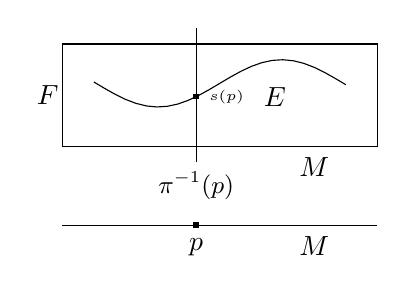
\begin{tikzpicture}[scale=1]
		\draw (-2,-0.3)--(2,-0.3)--(2,1)--(-2,1)--cycle;
		\node [label=left:$F$] (F) at (-1.8,0.35) {};
		\node [label=below:$M$] (M1) at (1.2,-0.2) {};
		\node [label=below:$M$] (M2) at (1.2,-1.2) {};
		\node [label=below:$E$] (E) at (0.7,0.7) {};
		\draw (-2,-1.3)--(2,-1.3);
		\node [fill=black, inner sep=1pt, label=below:$p$] (p) at (-0.3,-1.3) {};
		\draw [color=black, domain=-1.6:1.6] plot (\x,{0.3*sin(2*\x r)+0.5});
		%0.5-0.3*sin(0.6)=0.330607...
		\node [fill=black, inner sep=1pt, label=right:\tiny$s(p)$] (s) at (-0.3,0.3306) {};
		\draw (-0.3,-0.5)node[below]{\small$\pi^{-1}(p)$}--(-0.3,1.2);
	\end{tikzpicture}
	\caption{Trivial Bundle and its Section}
\end{figure}

\begin{pro}\label{pro:1.5.2}
	设$F\to E\xrightarrow{\pi}M$是一个纤维丛,则存在一个有限开覆盖$\{U_i\}$使得$\pi^{-1}(U_i)$同胚于平凡丛。
\end{pro}

这就意味着,纤维丛总是可以选一个有限图册(实际上,只需要$m+1$张坐标卡就行,其中$m$为流形$M$的维度)。

\begin{proof}
	设$\{(U_\alpha,\varphi_\alpha)\}$是$E$的一个图册,由于流形$M$的拓扑维数有限
	\footnote{设$X$是一个拓扑空间 $X$,如果对 $X$ 任意的一个开覆盖 $\{U_i\}$,都存在其一个开加细 $\{V_i\}$,使得$X$的每个点$x$都只属于至多 $n+1$ 个 $\{V_i\}$
	的元素,则定义$X$的拓扑维数为$n$. 不加证明地指出,$n$维流形的拓扑维数有限(实际为$n$),这可以通过将流形嵌入到欧式空间(通过单位分解)完成。},设为$m$,我们可以找一个$\{U_\alpha\}$的开加细,进而得到一个新的图册,其中任取$m+2$个开集相交都是空集。我们还是将这个图册记作$\{(U_\alpha,\varphi_\alpha)\}_{\alpha\in I}$.

	现在,找一个从属于$\{U_\alpha\}$的单位分解\footnote{见Lemma \ref{POU},在这里,如有必要,可以将$\{U_\alpha\}$换成Lemma \ref{POU}证明中构造的局部有限开加细。}$\{h_\alpha\}$. 若$S$是指标集$I$的有限子集,定义
	\[
		U_S=\{x\in M\,:\, \min_{\alpha\in S}h_{\alpha}(x)>\max_{\beta\not\in S}h_\beta(x)\}.
	\]
	此时,不难检验$\{U_S\}$是一个$M$的开覆盖,其中$S$跑遍$I$的有限子集。
	实际上,任取$x\in M$,我们知道其最多包含于$m+1$个$U_\alpha$中,将他们取作$S$,并在其中去掉所有使得$h_{\alpha}(x)=0$的$\alpha$,则此时,$\max_{\beta\not\in S}h_\beta(x)=0$,而$\min_{\alpha\in S}h_{\alpha}(x)>0$.
	所以$x\in U_S$. 此外,容易看出当$|S|>m+1$时,$U_S=\varnothing$,因为此时$\min_{\alpha\in S}h_{\alpha}(x)$总是为零,而从$\sum_{\beta\in I}h_\beta(x)=1$可知右侧必然不为零。

	最后,对正整数$k\geq 1$,定义
	\[
		U_k=\bigcup_{|S|=k}U_S,
	\]
	显然$\{U_k\}$是一个有限开覆盖,因为当$k>m+1$时$U_k=\varnothing$,下面我们证明$\pi^{-1}(U_k)$是平凡丛。首先注意到,若$\alpha\in S$,则$U_S\in U_\alpha$. 再注意到,如果$|S|=|T|$但$S\neq T$,则$U_S\cap U_T=\varnothing$. 实际上,如果$S\neq T$,其必然存在$\alpha\in S$, $\beta\in T$使得$\alpha\not\in T$, $\beta\not\in S$. 此时,如果
	$x\in U_S\cap U_T\neq \varnothing$,则从$x\in U_S$我们知道$h_{\alpha}(x)>h_\beta(x)$,从$x\in U_T$我们知道$h_{\beta}(x)>h_\alpha(x)$,矛盾。
	所以$U_k$实际上是一族不交并,而
	\[
		\pi^{-1}(U_k)=\bigcup_{|S|=k}\pi^{-1}(U_S)
	\]
	也是一族不交并。于是,我们可以通过
	\[
		\varphi_k|_{\pi^{-1}(U_S)}=\varphi_{\alpha}|_{\pi^{-1}(U_S)}
	\]
	将$U_S\subset U_\alpha$上的平凡化$\varphi_{\alpha}|_{\pi^{-1}(U_S)}$直接拼成$\pi^{-1}(U_k)$上的平凡化$\varphi_k$.
\end{proof}

\begin{para}[转移函数]
如果我们对纤维丛的同一个局部选取图册中不同的元素,比方说,在$U_\alpha$上有同胚$\varphi_\alpha=(\pi,\Phi_\alpha):\pi^{-1}(U_\alpha)\to U\times F$,在$U_\beta$上有同胚$\varphi_\beta=(\pi,\Phi_\beta):\pi^{-1}(U_\beta)\to U\times F$. 于是对所有$p\in U_\alpha\cap U_\beta$,
\[
	\Phi_{\alpha}|_{\pi^{-1}(p)}:\pi^{-1}(p)\to F\quad \text{and}\quad \Phi_{\beta}|_{\pi^{-1}(p)}:\pi^{-1}(p)\to F
\]
都是同胚。以后我们记对应的同胚$\Phi_{\alpha}|_{\pi^{-1}(p)}:\pi^{-1}(p)\to F$为$\Phi_\alpha(p)$,于是
\[
	\varphi_{\alpha\beta}(p):=\Phi_{\alpha}(p)\Phi_{\beta}(p)^{-1}:F\to F
\]
是一个同胚,满足
\begin{compactenum}
	\item $\varphi_{\alpha\alpha}(p)=\id_F$;
	\item $\varphi_{\alpha\beta}(p)\varphi_{\beta\alpha}(p)=\id_F$;
	\item $\varphi_{\alpha\beta}(p)\varphi_{\beta\gamma}(p)\varphi_{\gamma\alpha}(p)=\id_F$.
\end{compactenum}
这族同胚$\{\varphi_{\alpha\beta}\}$被称为纤维丛的转移函数族。不难检验,给定流形上的转移函数族,我们可以反过来构造一个纤维丛,这点在下面陈述$G$-丛构造定理的时候会有体现。
\end{para}

\begin{lem}
设$\pi:E\to M$是一个纤维丛,则$\pi$是一个淹没。
\end{lem}

只要验证,任取$e\in E$,$\pi_{*e}$都是满射即可,而这直接来自于局部平凡化。

\begin{para}[截面]
设$F\to E\xrightarrow{\pi} M$是一个纤维丛,$U\subset M$是一个开集,则$U$上的光滑截面(section)定义为一个光滑映射$s:M\to E$满足$\pi\circ s=\id_U$. $U$上所有截面的集合通常记做$\Gamma(U,E)$,如果$E$是清楚的,会直接写作$\Gamma(U)$. 
\end{para}

作为例子,考虑平凡从$M\times \mathbb{R}$,它的光滑截面是$M$上的光滑函数,因此,$M$上所有光滑函数的集合$\mathcal{C}^\infty(M)$就是$\Gamma(M\times \rr)$.

一个纤维丛不一定有整体截面,但是一定有局部截面(也可以直接用Lemma \ref{lem:2.9}),因为纤维丛在局部都是平凡丛,而平凡丛一定有截面,比如常值截面$s(x)=a\in F$. 对于一个纤维丛,直观来看,就是在底流形$B$每一点$p$,都放一个$\pi^{-1}(p)\cong F$,而所谓的截面,就是在每一点$p$,都选定$\pi^{-1}(p)\cong F$中的一个元素,这其实也就是矢量场的基本想法。对于切矢量场与余切矢量场,我们需要切丛与余切丛。

\begin{lem}[局部化原理]\label{localprin}
设$F\to E\xrightarrow{\pi} M$是一个纤维丛,$U$是$M$的一个开集,$\{U_\alpha\}$是$U$的一个开覆盖。再设$\{\sigma_\alpha\in \Gamma(U_\alpha,E)\}$是一族截面,满足在非空开集$U_\alpha\cap U_\beta$上$\sigma_\alpha|_{U_\alpha\cap U_\beta}=\sigma_\beta|_{U_\alpha\cap U_\beta}$. 则在$U$上存在唯一的光滑截面$\sigma$满足,$\sigma|_{U_\alpha}=\sigma_\alpha$.
\end{lem}

\begin{proof}
$\sigma$作为映射的构造是直接的,唯一需要注意的是光滑性,但是光滑性的检查是局部的,$\sigma$在局部都是$\sigma_\alpha$,所以是光滑的。
\end{proof}

作为推论,$U\mapsto C^\infty(U)$构成了一个$M$上的环层,我们记作$C^\infty_N$.

\begin{para}[切丛与余切丛]
流形$M$的\idx{切丛}(tangent bundle) $TM$被在集合上被定义为
\[
	TM=\bigsqcup_{x\in M}T_xM=\bigcup_{x\in M} \left\{x\right\}\times T_xM=\bigcup_{x\in M} \left\{(x, y)\vert\; y\in T_xM\right\}.
\]
\idx{余切丛}(cotangent bundle)$T^*M$在集合上被被定义为
\[
	T^*M=\bigsqcup_{x\in M}T^*_xM=\bigcup_{x\in M} \left\{x\right\}\times T^*_xM=\bigcup_{x\in M} \left\{(x, y)\vert\; y\in T_x^*M\right\}.
\]

通过把$(p,v)\in TM$映射到$p\in M$可以定义出映射$\pi: TM\to M$. 剩下的,我们要赋予$TM$一个光滑流形结构,然后检验是否满足纤维丛的定义。

为此,对于$p\in M$,找一个坐标卡$(U,\varphi)$,在这张卡内,$T_qM$通过$\varphi_{*q}$同构于$\rr^n$,我们这样选取$\pi^{-1}(U)$上的微分结构,使得他通过$\id_U\times \varphi_*$光滑同胚于$U \times \rr^n$,这样$TM$就有了一个坐标卡$(\pi^{-1}(U),\varphi\times \varphi_*)$,使得它构成了一个光滑流形,也是一个以$M$为底,$\rr^n$为纤维的纤维丛。同样地,$T^*M$也是一个纤维丛。
\end{para}

$TM$的截面即流形上的光滑矢量场,而$T^*M$的截面即流形上的光滑余切矢量场。

\begin{para}[丛映射]
设$F_1\to E_1\xrightarrow{\pi_1} M$和$F_2\to E_2\xrightarrow{\pi_2} M$都是$M$上的丛,如果映射$\varphi:E_1\to E_2$满足交换图
\[
	\xymatrix{
	E_1\ar[rr]^\varphi\ar[rd]_{\pi_1}&&E_2\ar[ld]^{\pi_2}\\
	&M&
	}
\]
则称$\varphi$为一个丛映射。
\end{para}

这里我们只考虑同一个流形上的两个丛之间的映射。特别地,任取$v\in \pi_1^{-1}(p)$,利用丛映射的性质,我们有$\pi_2\varphi(v)=\pi_1(v)=p$,即$\varphi(v)\in \pi_2^{-1}(p)$. 因此,$\varphi|_{(E_1)_p}:(E_1)_p\to (E_2)_p$. 换而言之,丛映射将同一点的纤维映射到同一点的纤维。

\begin{para}[拉回丛]
设$\pi:E\to N$是$N$上的一个纤维丛,而$f:M\to N$是一个光滑映射。那么纤维积$E\times_N M$,以及典范投影$\proj_M:E\times_N M\to M$就构成了一个$M$上的纤维丛。它被称为,丛$\pi:E\to N$沿着$f$的拉回丛,记作$f^*E$.
\end{para}

由于$\pi$是一个淹没,$\pi$和$f$自然横截相交,所以Proposition \ref{pro:2.21}告诉我们$f^*E$是$E\times N$的一个正则子流形。设$\varphi=(\pi,\Phi):\pi^{-1}(U)\to U\times F$是$U\subset N$上的局部平凡化,那么$f^{-1}(U)\subset M$上的局部平凡化写作$(\proj_M,\Phi\circ f)$. 于是,$E$上的丛结构给出了$f^*E$上的丛结构。特别地,纤维上有如下关系:$(f^*E)_{p}=E_{f(p)}$.

\begin{para}[$G$-丛]
设$G$是一个Lie群,$F\to E\xrightarrow{\pi} M$是一个纤维丛,它的图册为$\{(U_\alpha,\varphi_\alpha)\}$,以及$\lambda:G\times F\to F$是一个$G$在纤维上的光滑作用。如果在所有非空重叠开集上存在光滑映射$g_{\alpha\beta}:U_\alpha\cap U_\beta\to G$使得,任取$v\in F$,都有$\varphi_{\alpha\beta}(p)(v)=\lambda(g_{\alpha\beta}(p),v)$,且满足
\begin{compactenum}[~~~(1)]
	\item $g_{\alpha\alpha}(p)=e$;
	\item $g_{\alpha\beta}(p) g_{\beta\alpha}(p)=e$;
	\item $g_{\alpha\beta}(p) g_{\beta\gamma}(p) g_{\gamma\alpha}(p)=e$.
\end{compactenum}
此时,称$\{(U_\alpha,\varphi_\alpha)\}_{\alpha\in \Gamma}$是纤维丛$F\to E\xrightarrow{\pi} M$的一个$(G,\lambda)$-图册,而$F\to E\xrightarrow{\pi} M$被称为一个$(G,\lambda)$-丛。

通常会称$\{g_{\alpha\beta}\}$为覆盖$\{U_\alpha\}_{\alpha\in \Gamma}$的$G$-上链,上面的三个条件称为$G$-上链条件。映射$g_{\alpha\beta}:U_\alpha\cap U_\beta\to G$有时也被称为转移函数。如果作用$\lambda$在语境中没那么重要的,则称$F\to E\xrightarrow{\pi} M$是一个$G$-丛。
\end{para}

当$\lambda$是忠实作用的时候,对每一个转移函数,群元都是唯一确定的。此时我们可以从转移函数族的相关性质得到$G$-上链条件,即此时只需要满足$\varphi_{\alpha\beta}(p)(v)=\lambda(g_{\alpha\beta}(p),v)$即可。

\begin{thm}[$G$-丛构造定理]
	令$M$和$F$为光滑流形,$G$是一个Lie群。令$\{U_\alpha\}_{\alpha\in \Gamma}$是$M$的一个开覆盖,而$\{g_{\alpha\beta}\}$是一个$G$-上链。此时,任取一个纤维上的作用$\lambda:G\times F\to F$, 都存在一个$G$-丛,使得$\{(U_\alpha,\varphi_\alpha)\}$是其局部平凡化,且非空交集$U_\alpha\cap U_\beta$上满足$\varphi_{\alpha\beta}(p)(v)=\lambda(g_{\alpha\beta}(p),v)$. 
\end{thm}

\begin{proof}
	在不交并$\Sigma:=\bigsqcup_{\alpha\in \Gamma}U_\alpha\times F$上定义一个等价关系:$(p,y)\in U_\alpha\times F$等价于$(p',y')\in U_\beta\times F$ 当且仅当 $p=p'$ 和 $y=g_{\alpha\beta}(p)\cdot y'=\lambda(g_{\alpha\beta}(p),y')$. 从$G$-上链条件,不难检验这是良定的。
	
	我们的丛的全流形为$\Sigma/\!\!\sim$,它的元素是$\Sigma$中的等价类$\epsilon$. 定义$\pi:(p,y)\mapsto p$以及$\varphi_\alpha(\epsilon)$为$U_\alpha\times F$中满足$[p,y]:=(p,y)/\!\!\sim\,\,\in \epsilon$的唯一元素$(p,y)$. 此时,$F\to \Sigma/\!\!\sim\,\xrightarrow{\pi}M$就是我们需要的$G$-丛。
\end{proof}

下面我们介绍最重要的两个$G$-丛之一,矢量丛。另一个主丛将在后面介绍。

\begin{para}[矢量丛]
	设$\lambda$是一个Lie群$G$在矢量空间$V$上的(光滑)表示,则$(G,\lambda)$-丛$V\to E\xrightarrow{\pi} M$被称为纤维为$V$的矢量丛。

	设$V\to E\xrightarrow{\pi} M$是矢量丛,则在每条纤维$E_p:=\pi^{-1}(p)\cong V$上存在一个自然的矢量空间结构。实际上,假设$(U_\alpha,\varphi_\alpha)$ 是$p$附近的一个局部平凡化,$a$是一个标量,$s$, $t\in \pi^{-1}(p)$,我们能定义
	\[
	s+t:=\Phi_{\alpha}|_{E_p}^{-1}\left(\Phi_{\alpha}|_{E_p}(s)+\Phi_{\alpha}|_{E_p}(t)\right),\quad a\cdot s:=\Phi_{\alpha}|_{E_p}^{-1}\left(a\Phi_{\alpha}|_{E_p}(s)\right).
	\]
	这是良定的,如果$(U_\beta,\varphi_\beta)$是$p$附近的另一个局部平凡化,则
	\[
	\begin{aligned}
	\Phi_{\alpha}|_{E_p}^{-1}\left(\Phi_{\alpha}|_{E_p}(s)+\Phi_{\alpha}|_{E_p}(t)\right)&=\varphi_\beta|_{E_p}^{-1}\varphi_{\beta\alpha}(p)\left(\Phi_{\alpha}|_{E_p}(s)+\Phi_{\alpha}|_{E_p}(t)\right)\\
	&=\Phi_\beta|_{E_p}^{-1}\lambda\left(g_{\beta\alpha}(p),\Phi_{\alpha}|_{E_p}(s)+\Phi_{\alpha}|_{E_p}(t)\right)\\
	&=\Phi_\beta|_{E_p}^{-1}\left(\lambda\left(g_{\beta\alpha}(p),\Phi_{\alpha}|_{E_p}(s)\right)+\lambda\left(g_{\beta\alpha}(p),\Phi_{\alpha}|_{E_p}(t)\right)\right)\\
	&=\Phi_\beta|_{E_p}^{-1}\left(\varphi_{\beta\alpha}(p)\Phi_{\alpha}|_{E_p}(s)+\varphi_{\beta\alpha}(p)\Phi_{\alpha}|_{E_p}(t)\right)\\
	&=\Phi_\beta|_{E_p}^{-1}\left(\Phi_{\beta}|_{E_p}(s)+\Phi_{\beta}|_{E_p}(t)\right).
	\end{aligned}
	\]
	对于$a\cdot s$的检查也是类似的。

	反过来,设$V\to E\xrightarrow{\pi} M$是一个纤维丛,而$V$是一个矢量空间, 如果转移映射都是$V$上的线性映射,那么它们自然满足$G$-上链条件,其中$G$是$\operatorname{GL}(V)$的一个子群。从$G$-丛构造定理,$V\to E\xrightarrow{\pi} M$是一个$G$-矢量丛,而表示就是标准表示。
\end{para}

下面这个定义与上面的定义显然等价,也更加常见一些。

\begin{pro}
设$V\to E\xrightarrow{\pi} M$是一个纤维丛,图册为$\{(U_\alpha,\varphi_\alpha)\}$. 如果每条纤维$\pi^{-1}(p)=E_p$都有一个矢量空间结构,且对任意一个包含$p\in M$的$U_\alpha$,$\varphi_{\alpha}|_{E_p}:E_p\to V$都是线性同构,则$V\to E\xrightarrow{\pi} M$是一个矢量丛。
\end{pro}

所以,切丛和余切丛就是很清楚的矢量丛。

% \begin{para}
% 	对于矢量丛,给出一个局部平凡化等价于给出一族处处线性无关局部常值截面。所谓的常值就是说,$\varphi\circ s$到纤维$V$中的投影是一个常函数。显然,
% 	给出一个平凡化,我们可以找到一族处处线性无关局部常值截面。反过来,
% 	给出$U$上的一族处处线性无关的截面,我们可以定义
% \end{para}

\begin{para}[主$G$-丛]
一个主$G$-丛是一个纤维丛$G\to P\xrightarrow{\pi}M$,图册为$\{(U_\alpha,\varphi_\alpha)\}$,$G$是一个Lie群,并且,存在一个自由的右作用($g\in G$在$p\in P$上的右作用写作$pg$)满足
\begin{compactenum}[~~~~(1)]
	\item 对所有的$u\in P$, $g\in G$,$\pi(u)=\pi(ug)$;
	\item 对给定的局部平凡化$\varphi_\alpha=(\pi,\Phi_\alpha):\pi^{-1}(U_\alpha)\to U_\alpha\times G$使得
	\[
	\Phi_\alpha(u)g=\Phi_\alpha(ug)
	\]
	对所有$u\in \pi^{-1}(U_\alpha)$和$g\in G$都成立。
\end{compactenum}
\end{para}

\begin{lem}
主丛的纤维正好就是右作用的轨道。此外,对给定的$p$,$\Phi_{\alpha}(u)\Phi_{\beta}(u)^{-1}$是一个常值,其中$u\in \pi^{-1}(p)$,我们将其记作$g_{\alpha\beta}(p)$.
\end{lem}

\begin{proof}
	固定$p\in M$. 一方面,任取$u\in\pi^{-1}(p)$以及$g\in G$,则$\pi(ug)=\pi(u)=p$告诉我们$ug\in \pi^{-1}(p)$. 
	另一方面,任取$u$, $v\in\pi^{-1}(p)$,存在$p$的一个开邻域$U\subset M$使得
	\[
	\varphi=(\pi,\Phi):\pi^{-1}(U)\to U\times G,
	\]
	于是$\Phi(u)$, $\Phi(v)\in G$. 令$g=\Phi(v)^{-1}\Phi(u)$,于是
	\[
	\varphi(u)=(p,\Phi(u))=(p,\Phi(v)g)=(\pi(v),\Phi(vg))=(\pi(vg),\Phi(vg))=\varphi(vg).
	\]
	因为$\varphi$是双射,于是$u=vg$.

	此外,直接计算
	\[
		\Phi_{\alpha}(ug)\Phi_{\beta}(ug)^{-1}=\Phi_{\alpha}(u)gg^{-1}\Phi_{\beta}(u)^{-1}=\Phi_{\alpha}(u)\Phi_{\beta}(u)^{-1}.
	\]
	此即所证。
\end{proof}

作为流形,显然$M\cong P/G$.

\begin{pro}\label{pro:8}
主$G$-丛$G\to P\xrightarrow{\pi}M$是一个$(G,\mu)$-丛,其中$\mu$是Lie群上的左乘,转移函数为$g_{\alpha\beta}(p)=\Phi_{\alpha}(u)\Phi_{\beta}(u)^{-1}$,其中$u\in \pi^{-1}(p)$. 具体些说,即成立
\[
	\varphi_{\alpha\beta}(p)(g)=g_{\alpha\beta}(p)g.
\]
\end{pro}

\begin{proof}
	令$\left(\Phi_{\beta}|_{\pi^{-1}(p)}\right)^{-1}(g)=u$,于是$g=\Phi_\beta(u)$以及$\Phi_{\alpha}|_{\pi^{-1}(p)}\circ \left(\Phi_{\beta}|_{\pi^{-1}(p)}\right)^{-1}(g)=\Phi_{\alpha}(u)$. 另一方面,从$u\in \pi^{-1}(p)$
	\[
		g_{\alpha\beta}(p)g=\Phi_{\alpha}(u)\Phi_{\beta}(u)^{-1}\Phi_\beta(u)=\Phi_{\alpha}(u)=\Phi_{\alpha}|_{\pi^{-1}(p)}\circ \left(\Phi_{\beta}|_{\pi^{-1}(p)}\right)^{-1}(g).
	\]
	所以$\varphi_{\alpha\beta}(p)(g)=g_{\alpha\beta}(p)g$.
\end{proof}

下一个命题告诉我们,上一个命题给出了主$G$-丛的完整刻画。

\begin{pro}
如果$G\to P\xrightarrow{\pi}M$是一个$(G,\lambda)$-丛,$\lambda$在这里就是Lie群的左乘,则$G\to P\xrightarrow{\pi}M$是一个主$G$-丛。
\end{pro}

\begin{proof}
定义$ug=\varphi_{\alpha}^{-1}(p,\Phi_{\alpha}(u)g)$,其中$p=\pi(u)$. 这是良定的。假设$\varphi_\beta$是另一个局部平凡化映射,于是$\varphi_\beta(ug)=(p,\Phi_{\beta\alpha}(u)\Phi_\alpha(u)g)=(p,\Phi_{\beta}(u)g)$. 因此$\pi(ug)=\pi(u)$以及$\Phi_{\alpha}(ug)=\Phi_{\alpha}(u)g$,所以$G\to P\xrightarrow{\pi}M$是一个主$G$-丛。
\end{proof}

% As a corollary, in $(G,\lambda)$-vector bundle $(E,M,\pi,V)$, if $G$ is a subgroup of general linear group of $V$ and $\lambda$ is the standard representation, then $(E,M,\pi,V)$ is a principal $G$-bundle.

\begin{thm}
If $\pi:P\to M$ is a surjective submersion and a Lie group G acts freely on $P$ so that for each $p\in M$ and orbit of $p$ is exactly $\pi^{-1}(p)$, then $(P,M,\pi,G)$ is a principal $G$-bundle.
\end{thm}

\begin{proof}
	Without loss of generality, we can assume that the action is right action, since if it is a left action, we can define an equivalent right action by $p\cdot g:=g^{-1}p$.
	
	Since $\pi$ is a surjective submersion, for each $p\in M$, there exists a open neighbourhood $U\subset M$ and a local section $\sigma:U\to P$. Consider the map $f_\sigma:U\times G\to \pi^{-1}(U)$ given by $f_\sigma(p,g)=\sigma(p)g$. It is injective. If $\sigma(p)g=\sigma(p')g'$ is on the same orbit, then $\pi(\sigma(p)g)=p$ tell us $p=p'$, and $\sigma(p)g=\sigma(p)g'$ gives that $g=g'$ since the action is free. It is surjective, too. For each $u\in \pi^{-1}(U)$, $\sigma(\pi(u))\in \pi^{-1}(\pi(u))$, then there exists a $h\in G$ such that $u = \sigma(\pi(u))h$ since the orbit of $\pi(u)$ is exactly $\pi^{-1}(\pi(u))$, thus $u= f_\sigma(\sigma(\pi(u)),h)$.
	
	Now, suppose $\gamma(t)$ is a smooth curve on $\pi^{-1}(U)$ and $\gamma(0)=\sigma(p)g$, since the action is free, we can find a curve $g(t)$ on $G$ such that $\gamma(t)=\sigma(\pi(\gamma(t)))g(t)$. Let us define a linear map $\varphi_\sigma: T_{\sigma(p)g}P\to T_{p}M\oplus T_{g}G$ by $\gamma'(0) \mapsto (\pi\circ \gamma)'(0)\oplus g'(0)$, it is not difficule to vertify that it is the inverse of $(f_\sigma)_{*(p,g)}$. By inverse function theorem, bijection $f_\sigma:U\times G\to \pi^{-1}(U)$ is a local diffeomorphism, and then it is a diffeomorphism.
	
	Let $\varphi:=f_\sigma^{-1}$, then we have $\varphi=(\pi,\Phi)$ for a uniquely determined smooth map $\Phi:U\to G$. If $p=\pi(u)$, we have $\varphi(ug)=(p,\Phi(ug))$ and so
	\[
		ug=\varphi^{-1}(p,\Phi(ug)),
	\]
	while
	\[
	\begin{aligned}
		\varphi^{-1}(p,\Phi(u)g)&=f_\sigma(p,\Phi(u)g)=\sigma(p)(\Phi(u)g)=(\sigma(p)\Phi(u))g\\
		&=f_\sigma(p,\Phi(u))g=\varphi^{-1}(p,\Phi(u))g=ug=\varphi^{-1}(p,\Phi(ug)).
	\end{aligned}
	\]
	Since $\varphi^{-1}$ is a bijection, we have $\Phi(ug)=\Phi(u)g$. Thus the 	section $\sigma$ give rise to a principal bundle chart $(U,\varphi)$, where $\varphi=(\pi,\Phi)$.
\end{proof}

\begin{para}[Associated bundle]\label{11}
	Let $\pi:P\to M$ is a principal $G$-bundle, and suppose we are given a smooth left action $\lambda:G\times F\to F$ on a smooth manifold $F$. Then we can construct a $G$-bundle with base space $M$ and fiber space $F$ as follow.

	Define a right action of $G$ on $P\times F$ according to
	\[
	(u,y)g:=(ug,g^{-1}y)=(ug,\lambda(g^{-1},y)).
	\]
	The total space of our new bundle is the orbit space of this action $P\times_G F$. Denote the equivalence class of $(u,y)$ by $[u,y]$, and define $\bar{\pi}([u,y]):=\pi(u)$. $\bar{\pi}$ is a well-defined map because $\bar{\pi}([ug,g^{-1}y])=\pi(ug)=\pi(u)$. By the next lemma, we call bundle $(P\times_G F,M,\bar{\pi},F)$ the associated $G$-bundle of principal bundle $P$. 
\end{para}

If $\lambda$ is more important in the context, we usually use $P\times_\lambda F$ to denote the total space of associated bundle.

\begin{lem}
	$(P\times_G F,M,\bar{\pi},F)$ is a $G$-bundle with transition maps $\{\lambda(g_{\alpha\beta},*)\}$, where $g_{\alpha\beta}$ is the transition map of principal $G$-bundle $\pi:P\to M$.
\end{lem}

\begin{proof}
	Let $\{(U_\alpha,\varphi_\alpha)\}$ be a principal bundle atlas for $\pi:P\to M$. Note that $[\pi^{-1}(U_\alpha)\times F]=\pi^{-1}(U_\alpha)$. For each $\alpha$, define $\bar{\Phi}_\alpha:\pi^{-1}(U_\alpha)\to F$ by requiring that $\bar{\Phi}_\alpha([u,y])=\Phi_\alpha(u)\cdot y$ for all $[u,y]\in \pi^{-1}(U_\alpha)$ and then let $\bar{\varphi}_\alpha:=(\pi,\bar{\Phi}_\alpha)$ on $\pi^{-1}(U_\alpha)$. We want to show that $\bar{\varphi}_\alpha$ is bijective by defining an inverse for $\bar{\varphi}_\alpha$. For every $p\in U_\alpha$, let $\sigma_\alpha(p):=\varphi_\alpha^{-1}(p,e)$, where $e$ is the identity element in $G$. Then we have
	\[
	\sigma_\alpha(p) \cdot \Phi_\alpha(u)=\varphi_\alpha^{-1}(p,e)\cdot \Phi_\alpha(u)=\varphi_\alpha^{-1}(p,\Phi_\alpha(u))=u.
	\]
	Define $\eta_\alpha:U_\alpha\times F\to \pi^{-1}(U_\alpha)$ by $\eta_{\alpha}(p,y):=[\sigma_\alpha(p),y]$. We have
	\[
	\eta_\alpha\bar{\varphi}_\alpha([u,y])=\eta_\alpha(p,\Phi_\alpha(u)\cdot y)=[\sigma_\alpha(p),\Phi_\alpha(u)\cdot y]=[\sigma_\alpha(p)\cdot \Phi_\alpha(u),y]=[u,y].
	\]
	Thus $\eta_\alpha$ is a left inverse for $\bar{\varphi}_{\alpha}$. It is easily checked that $\eta_\alpha$ is also a right inverse for $\bar{\varphi}_{\alpha}$. Thus $\bar{\varphi}_\alpha$ is a bijection. Next we check the overlaps. We use Lemma \ref{pro:8};
	\[
	\begin{aligned}
	\bar{\varphi}_{\alpha}\bar{\varphi}_{\beta}^{-1}(p,y)&=\bar{\varphi}_{\alpha}\eta_\beta(p,y)=\bar{\varphi}_{\alpha}([\sigma_\beta(p),y])\\
	&=(p,\Phi_\alpha(\sigma_\beta(p))\cdot y)=(p,\Phi_\alpha(\varphi_\beta^{-1}(p,e))\cdot y)\\
	&=(p,\Phi_\alpha|_p\circ \Phi_\beta|_p^{-1}(e)\cdot y)\\
	&=(p,g_{\alpha\beta}(p)\cdot e\cdot y)\\
	&=(p,g_{\alpha\beta}(p)y).
	\end{aligned}
	\]
	This shows that the transition mappings  have the stated form and that the overlap maps $\bar{\varphi}_{\alpha}\bar{\varphi}_{\beta}^{-1}$ are smooth. The family $\{(U_\alpha,\bar{\varphi}_\alpha)\}$ provides the induced smooth structure and is also a bundle atlas.
\end{proof}

According to the above proof, the local trivializations of this bundle is $\bar{\varphi}_\alpha([u,y])=(\pi(u),\Phi_\alpha(u)y)$.

\begin{para}\label{13}
	Suppose that $(E,M,\pi,F)$ is a $G$-bundle, then it has a $G$-atlas $\{(U_\alpha,\varphi_\alpha)\}$ with associated $G$-valued cocycle of transition functions $\{g_{\alpha\beta}\}$. Using $G$-bundle construction theorem, one may construction a bundle with typical fiber $G$ by using left translation as the action. The resulting bundle is then a principal bundle $(P,M,\pi',G)$, and it turns out that $P\times_G F$ is equivalent to the original bundle $E$.
\end{para}

\begin{para}
	Suppose $F=V$ is a real (complex) vector space, and $\lambda:G\to \mathrm{GL}(V)$ is a representation of $G$ on $V$. Then $P\times_\lambda V$ has a natural vector bundle structure.
\end{para}

\begin{para}[仿射空间]
	设$V$是一个矢量空间,而$A$是一个集合,而$\lambda$是一个$V$作为加法群在$A$上的自由可迁(一般是右)作用,此时称$(A,V,\lambda)$是一个仿射空间。时常会直接将$A$称作仿射空间,而$V$被称为底空间,作用直接记作加法。

	设$A$和$A'$都是仿射空间,而$V$和$V'$是对应的底空间。设$f:A\to A'$是一个映射,任取$a\in A$,$V\in V$,由于作用是可迁的,所以存在一个唯一的$w\in A'$使得$f(a+v)=f(a)+w$. 这个$w$是$a$和$v$的函数,如果$w$不依赖于$a$且线性依赖于$v$. 则称$f$是一个仿射映射。从定义,$w$可以写为一个线性变换$[f]:V\to V'$作用在$v$上的结果,所以我们有$f(a+v)=f(a)+[f]v$.

	所有$A\to A$的可逆仿射变换(或称仿射同构)显然构成一个群,记作$\operatorname{GA}(A)$. 类似于表示,群$G$到$\operatorname{GA}(A)$的一个同态被称为$G$在$A$上的一个仿射表示。由于
	\[
		fg(a+v)=f(g(a)+[g]v)=fg(a)+[f][g]v,
	\]
	所以$[fg]=[f][g]$,这就意味着,存在一个典范同态$\operatorname{GA}(A)\to \operatorname{GL}(V)$. 特别地,每一个$G$的仿射表示$\lambda$都定义了一个表示$[\lambda]:g\mapsto [\lambda(g)]$.
\end{para}

每个矢量空间都是一个仿射空间,上面的仿射映射都可以写作$f(v)=f(0)+[f]v$,即一个线性变换加上一个平移,如果$f(0)=0$,则仿射映射就变成了线性映射。此时,仿射变换的复合写作
\[
	gf(v)=g(f(0)+[f]v)=g(0)+[g]f(0)+[g][f]v.
\]

\begin{para}[仿射丛]
	类似于矢量丛,我们可以定义仿射丛。设$A$是一个仿射空间,底矢量空间为$V$,	设$\lambda$是一个Lie群$G$在仿射空间$A$上的(光滑)仿射表示,则$(G,\lambda)$-丛$A\to E\xrightarrow{\pi} M$被称为纤维为$A$的仿射丛。此外,由$G$-丛构造定理,我们可以定义出一个$(G,[\lambda])$-矢量丛。它被称为仿射丛的底矢量丛。
\end{para}

一般来说,我们也可以从矢量丛出发构造一个仿射丛,比方说如果一个纤维丛的纤维都是仿射空间,底矢量空间是对应矢量丛的纤维,并且转移函数都是仿射同构,那么它就是一个仿射丛。

\begin{para}[一阶jet丛]
	设$\pi:Y\to X$是一个纤维丛,记$V_yY=\ker\pi_{*y}\subset T_yY$,称之为垂直空间。所谓$Y$上的一阶jet丛$J^1Y$是一个仿射丛,它在点$y$的纤维是满足$\pi_{*y}\gamma=\operatorname{id}$的所有线性映射$\gamma:T_{\pi(y)}X\to T_yY$的集合,这个集合有一个自然的仿射(其实也是矢量)空间结构,而所有$T_{\pi(y)}X\to V_yY$的线性映射构成其底矢量空间。

	一阶jet丛也可以用等价类来构造:设$\varphi$和$\psi$都是$x\in X$附近的局部截面,我们定义等价关系如下:如果$\varphi(x)=\psi(x)$且$\varphi_{*x}=\psi_{*x}$,则$\varphi\sim \psi$. 不难检验这是一个等价关系,那么我们就定义丛$J^1Y$在点$y$的纤维为在点$\pi(x)$附近的局部截面的等价类的集合。
\end{para}

\begin{lem}
	设$\gamma\in (J^1Y)_y$,则$T_yY=\im\gamma\oplus V_yY$.
\end{lem}

\begin{proof}
	从$\pi_{*y}\gamma=\id$,$\ker \gamma=\{0\}$. 首先,设$w\in \im\gamma$是非零矢量,则存在非零矢量$v$使得$w=\gamma(v)$,利用$\pi_{*y}\gamma=\id$立得$\pi_{*y}w=v\neq 0$,所以$w\not\in  V_yY$. 这就意味着$\im\gamma\cap V_yY=\{0\}$. 所以,这两个空间的和也就是它们的直和是$T_yY$的一个子空间。为证明这就是$T_yY$,只需计算维度。

	由于$\ker \gamma=\{0\}$,所以线性代数基本定理告诉我们$\dim \im\gamma=\dim T_xX$. 依然是线性代数基本定理,$\dim T_yY=\dim \ker \pi_{*y}+\dim \im \pi_{*y}=\dim V_yY+\dim T_xX$,所以$\dim T_yY=\dim V_yY+\dim \im\gamma$. 这就告诉我们$T_yY=\im\gamma\oplus V_yY$.
\end{proof}

\begin{para}[Ehresmann联络]
	设$\pi:Y\to X$是一个纤维丛,$J^1Y$丛在$Y$上的(局部)截面被称为$Y$的一个(局部)Ehresmann联络。
\end{para}

传统的Ehresmann联络的定义是在每一点(光滑地)给定$T_yY$的一个直和分解,分解为一个横空间$H_yY$与垂直空间$V_yY$的直和,而上一个引理告诉我们,$J^1Y$丛的一个截面就给出了这样一族横空间的选取。

\section{矢量丛}

这节我们来谈一些矢量丛的相关构造,尤其是矢量丛的截面层。

\begin{para}[矢量丛映射]
	设$F_1\to E_1\xrightarrow{\pi_1} M$和$F_2\to E_2\xrightarrow{\pi_2} M$都是$M$上的矢量丛,而$\varphi:E_1\to E_2$是一个丛映射。如果任取$p\in M$,$\varphi|_{\pi_1^{-1}(p)}:\pi_1^{-1}(p)\to \pi_2^{-1}(p)$是一个线性映射,则称$\varphi:E_1\to E_2$是一个矢量丛映射。
	\end{para}
	
	\begin{para}[矢量丛的子丛]
		设$V\to E\xrightarrow{\pi} M$是一个矢量丛,图册为$\{(U_\alpha,\varphi_\alpha)\}$,那么,如果存在$V$的矢量空间$V'$以及$E$的子流形$E'$,使得在任意的局部平凡化$(U_\alpha,\varphi_\alpha)$中
		\[
			\varphi_\alpha(\pi^{-1}(U)\cap E')=U\times V',
		\]
		则$V'\to E'\xrightarrow{\pi|_{E'}}M$是一个矢量丛,它被称为$V\to E\xrightarrow{\pi} M$的一个子矢量丛,简称子丛。如果$\dim V'=l$,则称这是一个秩为$l$的子丛。
	\end{para}
	
	\begin{lem}\label{lem:1.5.16}
		如果$\rho:F\to E$是$M$上矢量丛之间的映射,则
		$
			\ker \rho=\bigsqcup_{x\in M}\ker (\rho_x)
		$
		是$F$的一个子丛。
	\end{lem}	
	
	\begin{proof}
		由于$\rho_x$是满的,所以可以选一组$F_x$的基$\{v_1,\dots,v_l,v_{l+1},\dots,v_n\}$使得$\{\rho_x(v_1),\dots,\rho_x(v_l)\}$是$\im \rho_x$的一组基。利用局部平凡化,我们可以找一个$x$的邻域$U$以及$U$上的一组常值截面$\sigma_i$
		使得$\sigma_i(x)=v_i$使得$\{\sigma_i\}$在$U$上处处线性无关。
		适当缩小$U$,
		我们总可以使$\{s_i=\rho\sigma_i\,:\, 1\leq i\leq l\}$在$U$上也处处线性无关。于是,我们可以将其他截面用光滑函数展开$s_j = f^i_{r}s_i$,
		其中$l+1\leq j\leq n$. 最后,考虑截面
		\[
			\tau_{k}=\sigma_{r+k}-f_{k}^i\sigma_i,
		\]
		其中$1\leq k\leq n-l$. 这就给出了$\ker \rho$在$U$上的一个平凡化。
	\end{proof}
	
	\begin{para}[矢量丛的直和与张量积]
	设$G_1$, $G_2$都是Lie群,那么$G_1\times G_2$自然也是一个Lie群,群乘法为
	\[
		(g_1,h_1)(g_2,h_2)=(g_1g_2,h_1h_2).
	\]
	设$M$是一个流形,$\{U_\alpha\}$是其开覆盖,$\{g^1_{\alpha\beta}\}$是它上面的$G_1$-上链,而$\{g^2_{\alpha\beta}\}$是它上面的$G_2$-上链。那么$\{(g^1_{\alpha\beta},g^2_{\alpha\beta})\}$是$M$上的一个$(G_1\times G_2)$-上链。
	
	现在,设$V_1\to E_1\xrightarrow{\pi_1}M$是$(G_1,\lambda_1)$-矢量丛,$V_2\to E_2\xrightarrow{\pi_2}M$是$(G_2,\lambda_2)$-矢量丛。考虑$V_1\oplus V_2$,我们可以考虑$G_1\times G_2$的直和表示$\lambda_1\oplus \lambda_2$,具体写出来即
	\[
		\lambda_1\oplus \lambda_2((g_1,g_2))(v_1\oplus v_2)=\lambda_1(g_1)v_1\oplus \lambda_1(g_2)v_2.
	\]
	那么$G$-丛构造定理告诉我们,存在一个$(G_1\times G_2,\lambda_1\oplus \lambda_2)$-丛$E$
	\[
		V_1\oplus V_2\to E\xrightarrow{\pi} M.
	\]
	这个丛被称为前面两个丛的直和。
	
	直和丛还可以如下定义:设$V_1\to E_1\xrightarrow{\pi_1}M$和$V_2\to E_2\xrightarrow{\pi_2}M$是矢量丛,定义$E_1\oplus E_2 = E_1\times_M E_2$,
	此时
	\[
		V_1\oplus V_2\to E_1\oplus E_2\xrightarrow{\pi_1\proj_{E_1}} M
	\]
	就是我们需要的矢量丛。
	
	% 从直和丛的构造,不同发现两个典范投影$E_1\oplus E_2\to E_1$和$E_1\oplus E_2\to E_2$,它们都是光滑的矢量丛映射。实际上,从第二种定义,这两个典范投影都可以理解为纤维积的典范投影。
	
	类似地,考虑$V_1\otimes V_2$,我们可以考虑$G_1\times G_2$的张量积表示$\lambda_1\otimes \lambda_2$,具体写出来即
	\[
		\lambda_1\otimes \lambda_2((g_1,g_2))(v_1\otimes v_2)=\lambda_1(g_1)v_1\otimes \lambda_1(g_2)v_2.
	\]
	那么$G$-丛构造定理告诉我们,存在一个$(G_1\times G_2,\lambda_1\otimes \lambda_2)$-丛$E'$
	\[
		V_1\otimes V_2\to E'\xrightarrow{\pi'} M.
	\]
	这个丛被称为前面两个丛的张量积。
	\end{para}
	
	\begin{para}[The dual bundle of a vector bundle]
		Suppose that $(E,M,\pi,V)$ is a $(G,\lambda)$-vector bundle, $V^*$ is the dual space of $V$, and $\lambda^*$ is the dual representation of $\lambda$ of $G$ on $V^*$ such that $\lambda^*(g)=\lambda(g^{-1})^*$. By \ref{13}, we could construct a principal bundle $(P,M,\pi',G)$ from $(E,M,\pi,V)$, and $P\times_{\lambda^*} V^*$ is a $(G,\lambda^*)$-vector bundle by \ref{11}. The vector bundle $P\times_{\lambda^*} V^*$ is often called the dual bundle of the vector bundle $E$, or dual bundle for short, written as $E^*$.
	\end{para}
	
	Similarily, suppose that $V^{m,n}$ is the tensor product $V^*\otimes \cdots \otimes V^*\otimes V \otimes \cdots \otimes V$. There's a natural representation $\lambda^{m,n}=\lambda^*\otimes \cdots \otimes \lambda^*\otimes \lambda \otimes \cdots \otimes \lambda$ of $G$ on $V^{m,n}$ induced from $\lambda$ on $V$. Thus, $P\times_{\lambda^{m,n}} V^{m,n}$ is a $(G,\lambda^{m,n})$-vector bundle, and it's often written as $E^*\otimes \cdots \otimes E^*\otimes E \otimes \cdots \otimes E$ or $E^{m,n}$ for short.
	
	% \begin{para}[Tensor product of vector bundles]
	% Suppose that $(E,M,\pi,V)$ is a $(G,\lambda)$-vector bundle, and $(E',M,\pi',V')$ is a $(G,\lambda')$-vector bundle. Then representation $\lambda\otimes \lambda' : G\to \mathrm{GL}(V\otimes V')$ defines a $(G,\lambda\otimes \lambda')$-vector bundle $(E\times E',M,\pi\times \pi',V\otimes V')$. 
	% \end{para}

	\begin{pro}
	任取$p\in M$,则存在矢量空间的典范同构:
	\[
		(E_1\oplus E_2)_p\cong (E_1)_p\oplus (E_2)_p,\quad (E_1\otimes E_2)_p\cong (E_1)_p\otimes (E_2)_p.
	\]
	\end{pro}
	
	有了这些典范同构,所以以后我们等同这些纤维。
	
	\begin{proof}
	直和和张量积的证明是类似的,所以我们只对张量积证明。给定$p$处的一个局$U$,在$E_1$, $E_2$和$E_1\otimes E_2$上面分别有局部平凡化映射$\varphi_1$, $\varphi_2$和$\varphi$. 此时
	\[
		\varphi|_{(E_1\otimes E_2)_p}:(E_1\otimes E_2)_p\to V_1\otimes V_2,
	\]
	\[
		\varphi|_{(E_1)_p}:(E_1)_p\to V_1,\quad \varphi|_{(E_2)_p}:(E_2)_p\to V_2
	\]
	都是线性同构。所以,存在线性同构
	\[
		\varphi|_{(E_1)_p}\otimes \varphi|_{(E_2)_p}:(E_1)_p\otimes (E_2)_p\to V_1\otimes V_2
	\]
	以及
	\[
		\varphi|_{(E_1\otimes E_2)_p}^{-1}\circ \left(\varphi|_{(E_1)_p}\otimes \varphi|_{(E_2)_p}\right):(E_1)_p\otimes (E_2)_p\to (E_1\otimes E_2)_p.
	\]
	这就是我们需要的同构。当然,我们还需要检验这与选取的平凡化无关:如果我们选取不同的局部平凡化,则$\varphi|_{(E_1)_p}\otimes \varphi|_{(E_2)_p}$中贡献一项$\lambda_1((g_1)_{\alpha\beta}(p))\otimes \lambda_2((g_2)_{\alpha\beta}(p))$,而$\varphi|_{(E_1\otimes E_2)_p}^{-1}$提供了相逆的一项,消去了这种不确定性。
	\end{proof}
	
	% \begin{lem}
	% 设$V$和$W$都是$M$上的矢量丛,则存在典范矢量丛映射$V\to V\otimes W$以及$W\to V\otimes W$.
	% \end{lem}
	
	% \begin{proof}
	% 两个丛映射的构造是类似的,所以只证明第一个。首先,$M$上存在开覆盖$\{U_\alpha\}$,在每一个$U_\alpha$上,$V$和$W$都可以局部平凡化,平凡化映射记作$\varphi^V_\alpha=(\pi^V,\Phi^V_\alpha)$和$\varphi^W_\alpha=(\pi^W,\Phi^W_\alpha)$. 那么,任取$a\in V$,我们可以
	% \end{proof}

\begin{para}[矢量丛的截面层]
	矢量丛的(光滑)截面被称为一个(光滑)矢量场。设$\pi:E\to M$是一个矢量丛,$\Gamma(U,E)$是$E$在$U$上所有光滑截面的集合。对矢量丛$E$,纤维$E_p$已知有自然的矢量空间结构,于是任取$f\in \mathcal C^\infty_M(U)$, $\sigma_1$, $\sigma_2\in \Gamma(U,E)$,可以逐点定义出两个新的截面
	\[
		f\sigma_1:p\mapsto f(p)\sigma_1(p),\quad \sigma_1+\sigma_2:p\mapsto \sigma_1(p)+\sigma_2(p),
	\]
	它们都是光滑的,所以$\Gamma(U,E)$有一个自然的$\mathcal C^\infty_M(U)$-模结构。
\end{para}
	
在通过前面提及过的局部化原理Lemma \ref{localprin},$U\mapsto \Gamma(U,E)$构成了一个层,同时也是$\mathcal C^\infty_M$-模层。

\begin{para}[矢量值截面]
	给定一个矢量丛$V\to E\xrightarrow{\pi} M$,还有一个矢量空间$W$. 对矢量空间$W$和流形$M$,我们可以构造出一个平凡的矢量丛$M\times W$. 那么我们定义丛$E\otimes W$为$V\to E\xrightarrow{\pi} M$和矢量丛$M\times W$的张量积。并且,定义$\Gamma(U,E;W)=\Gamma(U,E\otimes W)$,它的元素被称为一个$W$-值截面。
	\end{para}
	
	作为应用,设$V$是一个有限维矢量空间,则$\omega\in \Gamma(T^*M;V)$被称为一个$V$-值1-形式。在每一个纤维上,他有一个自然的矢量空间结构,于是$\Gamma(T^*M;V)$也构成了一个矢量空间。
	
	\begin{para}[Lie群的切丛]
	Lie群$G$的切丛$TG$相当简单,因为我们可以定义$(l_{a^{-1}})_*$把$T_aG$始终映射到$T_eG=\lag$来考虑,所以切丛就被平凡化了,它同构于$G\times \lag$. 与这相关的概念即Maurer-Cartan形式。设$G$是一个Lie群,他的切丛记做$TG$,映射$\omega_G:(g,v)\mapsto (l_{g^{-1}})_*v$被称为Maurer-Cartan形式。可以看到$\omega_G:\Gamma(TG)\to \lag$,因此Maurer-Cartan形式可以看做一个$\lag$-值1-形式,即$\omega_G\in \Gamma(T^*G;\lag)$. 且对于任意的$l_h^*$,我们都有
	\[
		(l_h^*\omega_G)v=\omega_G((l_h)_*v)=(l_{(hg)^{-1}})_*(l_h)_*v=(l_{(g)^{-1}})_*v=\omega_G(v).
	\]
	所以Maurer-Cartan形式是左不变的。
	
	特别地,一般线性群上面的Maurer-Cartan形式即为$\omega_G(v)=l_{g^{-1}}(v)=g^{-1}v$,其中$g$和$v$都是矩阵,矩阵乘矩阵还是矩阵,所以Lie代数$\mathfrak{gl}(n,\rr)$也是矩阵的形式。设$\dd g=(\dd x_{ij})$,那么$v$就可以写成$\dd g(v)$,因为$\dd x_{ij}(v)=v_{ij}$,则$\omega_G=g^{-1}\dd g$.
	\end{para}

\begin{pro}\label{pro:1.6.2}
	任何矢量丛都可以看成某个平凡矢量丛的子丛。更确切地说,对矢量丛$E$,存在一个矢量丛$E^\bot$使得$E\oplus E^\bot$是一个平凡矢量丛。
\end{pro}
		
平凡矢量丛就是同构于$M\times V$的矢量丛(同构是在丛映射意义下的),其中$V$是一个有限维矢量空间。

\begin{proof}
	设$V\to E\xrightarrow{\pi}M$是一个矢量丛,且$\dim V=n$. 
	那么,从Proposition \ref{pro:1.5.2}可知,存在一个有限图册$\{U_\alpha,\varphi_\alpha\}$,使得对每一个坐标卡,$\varphi_\alpha:\pi^{-1}(U_\alpha)\to U\times V$
	是一个同胚,同时可以找一个从属于开覆盖$\{U_{\alpha}\}$的
	单位分解$\{h_\alpha\}$(见Lemma \ref{POU}).

	对每一个$\alpha$,找一组在$U_\alpha$上处处线性无关的截面
	$s_\alpha^i$, $\dots$, $s_\alpha^n$,定义$\sigma_\alpha^i=h_\alpha s_\alpha^i$. 此时$\sigma_\alpha^i$都是整体截面,且在$U_\alpha$外为零。
	于是,对每个$x\in M$,$\{\sigma_\alpha^i(x)\}$张成了$E_x$. 现在,考虑
	有限维空间$V=\operatorname{span}_\rr (\{\sigma_\alpha^i\})$,以及平凡从$p:M\times V\to M$. 我们通过$\rho(x,\sigma)=\sigma(x)$定义一个映射
	\[
		\rho:M\times V\to E.
	\]
	显然这是光滑的,且它诱导纤维之间的满线性映射$\rho_x:(M\times V)_x\to E_x$. 所以这是一个矢量丛之间的映射,最后我们定义$E^\bot$为
	$F$的子丛$\ker \rho$(见Lemma \ref{lem:1.5.16}). 由于$\rho_x$处处是满射,所以我们有$E\oplus E^\bot\cong M\times V$.
\end{proof}

对于整体截面,$\Gamma(E\oplus E^\bot,M)=\Gamma(E,M)\oplus \Gamma(E^\bot,M)$,所以作为自由模的直和项,$\Gamma(E,M)$是一个$C^\infty_M(M)$-投射模。
实际上,Swan定理告诉我们,流形$M$上的有限秩的光滑矢量丛范畴和$C^\infty_M(M)$-投射模范畴等价,这里我们并不打算证明这点。

\begin{thm}
	设$E_1$和$E_2$都是$M$上的矢量丛,$E_1\otimes E_2$为这两个丛的张量积,则任取$M$上的开集$U$,$\Gamma(U,E_1\otimes E_2)$和$\Gamma(U,E_1)\otimes_{C^{\infty}_M(U)} \Gamma(U,E_2)$典范同构。
\end{thm}
	
	从$\Gamma(U,E_1)\times \Gamma(U,E_2)$到$\Gamma(U,E_1\otimes E_2)$的映射是不难定义的,实际上,给定$(\sigma_1,\sigma_2)\in \Gamma(U,E_1)\times \Gamma(U,E_2)$,则
	\[
		p\mapsto \sigma_1(p)\times \sigma_2(p)\in (E_1)_p\otimes (E_2)_p=(E_1\otimes E_2)_p
	\]
	给出了$\Gamma(U,E_1\otimes E_2)$中的一个截面。同时,不难检验对$C^{\infty}_M(U)$,这是双线性的。所以,从张量积的泛性质,存在一个$C^{\infty}_M(U)$-线性映射
	\[
		\alpha(U):\Gamma(U,E_1)\otimes_{C^{\infty}_M(U)} \Gamma(U,E_2)\to \Gamma(U,E_1\otimes E_2).
	\]
	他是同构的证明并不简单。
	
\begin{proof}
	首先,我们可以只考虑整体截面,此时我们将矢量丛的整体截面简记为$\Gamma(E)$. 容易看到,如果$E_1$, $E_2$都是平凡矢量丛,则定理是正确的。对于非平凡的矢量丛,我们应用Proposition \ref{pro:1.6.2},考虑如下交换图
	\[
	\begin{xy}
		\xymatrix{
		\Gamma(E_1) \otimes_{C^{\infty}_M(M)} \Gamma(E_2)\ar[r]^\alpha\ar[d]^i & \Gamma(E_1 \otimes E_2) \ar[d]^{j}\\
		\Gamma(E_1 \oplus E_1^{\perp}) \otimes_{C^{\infty}_M(M)} \Gamma(E_2 \oplus E_2^{\perp}) \ar[r]^{\alpha'}& \Gamma((E_1 \oplus E_1^{\perp}) \otimes (E_2 \oplus E_2^{\perp})) 
		}
	\end{xy}
	\]
	其中$i$, $j$为直和典范含入,而$\alpha$, $\alpha'$都是来自于张量积泛性质的典范映射,$E_1 \oplus E_1^{\perp}$和$E_2 \oplus E_2^{\perp}$都是平凡矢量丛。从平凡矢量丛的结论,$\alpha'$是同构,所以从$j\alpha=\alpha'i$是单射,可以知道$\alpha$是单射。类似地,将$i$, $j$换成直和的典范投影(箭头方向也反过来),则$\alpha'$是满射告诉我们$\alpha$也是满射。
\end{proof}

从今以后,让我们典范等同$\Gamma(U,E_1)\otimes_{C^{\infty}_M(U)} \Gamma(U,E_2)$和$\Gamma(U,E_1\otimes E_2)$. 作为等同的结果,我们有

\begin{pro}
	$\Gamma(E^{n,m},U)=\Gamma(E,U)^{n,m}$.
\end{pro}

作为例子,我们考虑Riemann度量。

\begin{para}[Riemann度量]
	设$M$是一个流形,$T^*M$是其余切丛,$T^*M\otimes T^*M$是余切丛与自己的张量积。取$g\in \Gamma(T^*M\otimes T^*M,M)$,在$M$的每一点$p$处,$g_p\in T^*_pM\otimes T^*_p M$. 如果任取$p\in M$,以及$v$, $w\in T_pM$,满足
	\begin{compactenum}[~~~~(1)]
	\item $g_p(v,w)=g_p(w,v)$;
	\item $g_p(v,v)\geq 0$;
	\item $g_p(v,v)=0$当且仅当$v=0$.
	\end{compactenum}
	则称$g$是流形$M$上的一个Riemann度量。

	显然,$g$还可以看作一个映射
	\[
		g:\Gamma(TM\otimes TM,M)=\Gamma(TM,M)\otimes_{C^\infty_M(M)} \Gamma(TM,M) \to C^\infty_M(M),
	\]
	这是因为$\Gamma(T^*M\otimes T^*M,M)=\Gamma(TM\otimes TM,M)^*$,其中的元素都是$\Gamma(TM\otimes TM,M)\to C^\infty_M(M)$的$C^\infty_M(M)$-线性函数。
\end{para}
	
	回忆,在$\rr^n$上有一个自然的Riemann度量,定义为$g_p(e_i,e_j)=\delta_{ij}$,其中$p\in \rr^n$, $\{e_i\}$为$\rr^n$的标准基。利用局部化原理,我们可以从一些开集上的$g$将其拼成一个整体的Riemann度量,而这给出了流形上Riemann度量存在性的证明。
	
	\begin{lem}
		流形上存在Riemann度量。
	\end{lem}
	
	\begin{proof}
		设$M$是一个流形,我们找一个图册$\{(U_\alpha,\varphi_\alpha)\}$,以及上面的单位分解$\{h_\alpha\}$(见Lemma \ref{POU})。对每一个坐标卡,我们可以利用同构$\varphi_\alpha:U_\alpha\to \rr^n$,将$\rr^n$上的自然的Riemann度量拉回到$U_\alpha$上,我们将其定义为$g_\alpha$,最后,定义$g=\sum_{\alpha}h_\alpha g_{\alpha}$,不难检验这是一个Riemann度量。
	\end{proof}
	
	\begin{para}[作为截面的推前]
	作为另一个例子,设$\varphi:M\to N$是一个流形间的光滑映射,如果$X$是$TM$的一个截面,那么通过
	\[
		\varphi_* X:p\mapsto \varphi_{*p}X_p\in T_{\varphi(p)}N=(\varphi^*TN)_p,
	\]
	可以看到$\varphi_* X$是拉回丛$\varphi^*TN$的一个截面(注意,这不是$N$上的矢量场)。于是,我们定义了一个映射
	\[
		\varphi_*:\Gamma(U,TM)\to \Gamma(U,\varphi^*TN).
	\]
	如果利用矢量场与1-形式之间的缩并,我们还有
	\[
		\varphi_*\in \Gamma(U,\varphi^*TN)\otimes_{C^\infty_M(U)} \Gamma(U,T^*M)=\Gamma(U,\varphi^*TN\otimes T^*M).
	\]
	\end{para}